\part{Characterising the beam} % (fold)
\label{prt:characterising_the_beam}
% TODO: Measurements:: Measurements: Characterising the beam: write me
\chapter{Introduction} % (fold)
\label{sec:measurements_introduction}

Characterisation of the MuSIC beam was carried out over several years and through a number of experiments. Over the course of five beam-times three significant measurements were made to characterise the beam: the total charged particle flux, the muon lifetime and the momentum spectrum; table~\ref{tab:summary_music_beam_time} covers the details. Several other experiments were also carried out although these are not discussed here.
\begin{table}[htpb]
  \begin{center}
  \begin{tabular}{c|c|c}
    \multicolumn{2}{c|}{Dates}          & Measurements                                \\
    Start            & Stop             &                                             \\
    \hline                                                                             
    29 July 2010     & 31 July 2010     & Charged particle flux.                      \\
    13 February 2011 & 16 February 2011 & Muon lifetime in Cu and Mg.                 \\
    19 July 2011     & 21 July 2011     & Muon yield (via lifetime).                  \\
                     &                  & Muon yield (via muonic X-rays).             \\
    22 October 2011  & 23 October 2011  & Neutron flux.                               \\
    18 June 2012     & 22 June 2012     & Muon momentum spectrum (via lifetime).      \\
                     &                  & Muon momentum spectrum (via muonic X-rays). \\
  \end{tabular}
  \end{center}
  \caption{A summary of the five MuSIC beam-times with notes on the measurements made.}
  \label{tab:summary_music_beam_time}
\end{table}
`'
\section{Experimental method} % (fold)
\label{sec:experimental_method}
All of the measurements discussed here use scintillators to measure the beam. As discussed in section~\ref{sec:charged_particle_interactions_in_matter} scintillators respond to ionisation by emitting photons. The number and spectrum of emitted photons depends on the amount of energy deposited and the characteristics of the material. A commonly quoted value for plastic scintillator's light yield is 1 photon per 100~eV of deposited energy~\cite{PDG particle detectors review}. 

To increase the proportion of light captured the scintillators were wrapped in mylar and then black-wrap. The combination of these two additional layers meant that any light exiting the scintillator would be reflected back in whilst external light was kept out to prevent background. The thickness of both the mylar and black-wrap were minimised in order to prevent excess energy loss in these layers.

Due to the large magnetic field present at the end of the beam large PMTs were not a viable option, instead a type of silicon photomultiplier (SiPM) called a `Multi-Photon Pixel Counter' (MPPC) was employed. Each MPPC is composed of an array of Avalanche Photodiodes (APD), an array typically contains between 100 and 1,600 individual APDs. An APD operates by maintaining a small region of doped silicon close to its breakdown voltage (for an MPPC this is \( \sim -\)70~V) when a photon is incident on this region an electron/hole pair is created via the photo-electric effect. The bias voltage is large enough to accelerate the electron/hole pair causing ionisation of the silicon and further pairs to be created. This `avalanche' of pairs has a gain of order \( 10^5 \), large enough (\( \sim \)25~mV) that with proper amplification and noise removal it can be detected.

The largest disadvantage to using MPPCs is that, due to their sensitivity, they're a noisy sensor. They typically have a false positive (the `dark count') rate of \( \mathcal{O}(150)\times10^3 \)~counts/s (cps). The dark count can be easily removed by rejecting low photon count events, a minimum voltage threshold of \( \sim 0.5\)~photo-electrons (p.e.) is used to measure the dark-count and, given the poisson-nature of the noise, a threshold of 1.5~p.e. will remove the majority of dark counts (\(\gtrsim60\%\)). 

% TODO Good example of MPPC signal

In order to make the actual measurements first the signals from the MPPCs had to be processed and then digitised. The exact details of this varied from measurement to measurement (and are discussed in the relevant chapters) the general process was always the same: first the signal is amplified, then it is determined if the signal is to be measured (triggering) and finally the signal is read out. 

Amplification of the signals was done to change the signal to one which was above the threshold of the discriminator units. The discriminator units normally had a minimum threshold of 10~mV with a minimum \emph{viable} (i.e.\ stable) threshold of \( \sim \)50~mv; the signals from an MPPC are generally \( \mathcal{O}(10) \)~mV obviously too small for the discriminators, even before any attenuation. In order to make the MPPC signals detectable the signal was amplified twice: first in the experimental hall and again at the DAQ-station, downstairs. 

Once the MPPC signal has been amplified suitably it is converted to a digital signal using a discriminator. The advantage of converting the analogue MPPC signal to a digital one is that the digital signal is much easier to manipulate and process, unfortunately there is a loss of information which has to be accounted for. Digitisation is done using a discriminator which is a device that receives an analogue input and sends a digital output. The digital output is sent (`asserted') when the input exceeds some pre-set threshold. Assuming that the input exceeds the discriminator's threshold for long enough to be detected (normally \(\gtrsim8\)~ns) the output will be asserted for as long as the input is or the pre-set minimum output width; which ever is longer. 

Whilst the MPPCs are all similar they are not identical so to account for variance in gain and inaccuracies in the analogue amplification discriminator thresholds were normalised to the number of photo-electrons that any particular voltage corresponded to. Setting the threshold was done using an oscilloscope to visualise the impact of any particular threshold by using the discriminator's output as the oscilloscope's trigger whilst plotting the analogue signal trace, an example of this can be seen in figure~\ref{fig:set_dis_thrs_for_mppc}.

\begin{figure}[hptb]
  \centering  
    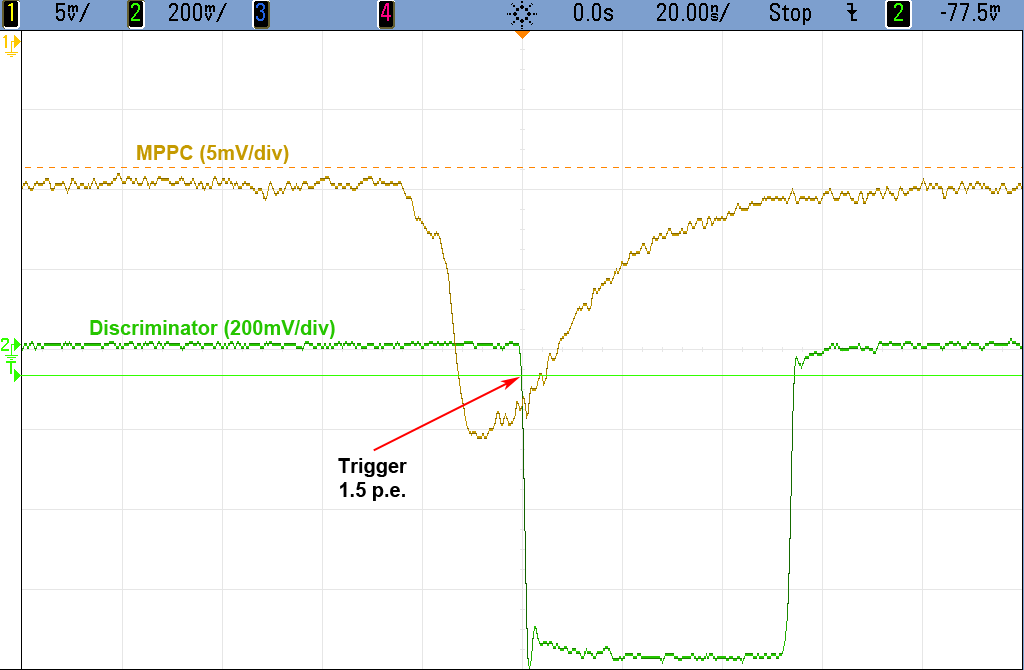
\includegraphics[width=.9\textwidth]{images/edit/scope_dis_ch_2.png}
  \caption{An example oscilloscope trace being used to set the discriminator threshold. In this case the threshold is set to \( \sim \)1.5~p.e. (i.e.\ \( \sim- \)15~mV). The discriminator signal being used to trigger is shown in green whilst the input MPPC signal is brown. There are 200~mV/div for the discriminator signal whilst the MPPC signal has 5~mV/div; the time resolution is 20~ns/div.}
  \label{fig:set_dis_thrs_for_mppc}
\end{figure}

Careful setting of the discriminator threshold removes the majority of noise from the signal it doesn't remove all of it, to account for this a more stringent requirement is placed upon signals from the MPPC: co-incidence across MPPCs. Whilst it's entirely possible for a burst of noise to mimic a signal of several photo-electrons in one MPPC it is highly unlikely for this to occur in more than one MPPC. The standard second stage of the DAQ is to require that all the MPPCs on a scintillator register a suitably strong (e.g.\ at least \( >1.5\)~p.e.) signal. The co-incidence requirement is also combined with any additional logic for the system, e.g.\ busy signals from the readout computer or anti-co-incidence with other scintillators. 

% TODO Calculate 

Anti-co-incidence is used heavily in the muon lifetime measurements. All the muons produced at MuSIC are travelling at a reasonable fraction of the speed of light, this means that scintillators with a suitably small separation (\( \mathcal{O}(10)\)~mm) will detect such a muons almost simultaneously. By placing a high density `stopping target' between two such scintillators it is possible to detect which muons have likely stopped by looking for a hit in the upstream scintillator and no corresponding hit in the downstream scintillator. 

% TODO probably want to split this into separate subsections, one per measurement device e.g. scaler, (PH)ADC and (MH)TDC as well as information on the modules used and CAMAC/NIM in general

As well as discrimination of the MPPC signals there are three other useful measurements to be made: counting the number of signals from the discriminator, measurement of the size of the MPPC signals and measurement of the timing difference between up and downstream scintillators (if used). Whilst the discriminator is a measurement of the signal size it has a very low information content, by using an Analogue to Digital Converter (ADC) it is possible to get a much more precise measurement of the either the peak potential (so called `Peak Height' or PH-ADC) of the signal or the integrated charge. For MPPCs the peak value of the potential is the most useful number so it is this that we measure. When two scintillators are used by measuring the time differences between an anti-co-incident hit in the upstream scintillator (and only the up-stream scintillator) and then subsequent hits in the downstream scintillator (after a suitable anti-co-incidence or veto window) it's possible to reconstruct the lifetime of the upstream particle, for this to work a Multi-Hit Time to Digital Converter (MH-TDC) is used. A MH-TDC is required as some number of the downstream hits will be noise (often electrons) the noise appears as a flat background whilst the signal, electrons produced in the decay of the upstream muon, are correlated with the start time through an exponential. 

% TODO figure out what SEC stands for
% TODO Add info on SEC proton current measurement
% TODO How well do we know the energy of the initial proton beam, especially at low energies? 
% TODO need info on why 380 MeV is pion production threshold
As well as measuring the properties of the muon beam in order to make reasonable measurements we need to understand the properties of the initial proton beam. The key value is the proton beam's current which defines the number of protons at the PCS and hence its efficiency. The proton beam's current is estimated during operation using a Secondary Emission Chamber (SEC). The SEC contains a thin gold foil that is connected to an ammeter enabling direct measurement of a fraction of the beam during a run. The exact fraction absorbed by the gold foil is determined during a calibration run in which the entire beam's current is measured using a copper block to absorb it.

% section experimental_method (end)
%%%%%%%%%%%%%%%%%%%%%%%%%%%%%%%%%%%%%%%%%%%%%%%%%%%

% chapter measurements_introduction (end)
%%%%%%%%%%%%%%%%%%%%%%%%%%%%%%%%%%%%%%%%%%%%%%%%%%%
\chapter{Charged Particle Flux} % (fold)
\label{sec:charged_particle_flux}
% TODO: Measurements:: Charged Particle Flux: write me
% TODO: Measurements:: Charged Particle Flux: cover scint design
% TODO: Measurements:: Charged Particle Flux: cover DAQ
% TODO: Measurements:: Charged Particle Flux: cover what happened
% TODO: Measurements:: Charged Particle Flux: Check dimensions & positions of 1D scint
% TODO: Measurements:: Charged Particle Flux: Check dimensions & positions of 2D scint
Two measurements of the charged particle flux were made: the first using a long strip of scintillator (380\(\times\)30\(\times\)8~mm) positioned across the face of the beam pipe at a variety of heights; the second measurement was made using a \(35\)~mm radius \( 20 \)~mm deep disk. 

Both measurements were made using a scaler to count the raw trigger rate, which was recorded with the beam both on and off. The raw trigger rate is defined as a signal from all MPPCs that passes discrimination. To normalise the trigger rate between runs the proton beam intensity was measured using SEC.

% TODO check distance from beampipe
The vertical measurements were made \( 50 \)~mm from the end of the MTS at: \( -15 \), \( -5 \), \( 0 \), \( +5 \) and \( +15 \)~mm, measured from the centre of the beam-pipe. For each position both the SEC and trigger rate were measured with the beam on, and then to measure the bias measured off. Each value was measured for 50~s.

% To make the measurement to values were recorded: the total trigger rate (i.e.\ the number of charged particles) and the intensity (i.e.\ current) of the proton beam (for normalisation). A trigger was defined as an all-MPPC co-incidence above the discriminator threshold. Measurement of the pro
\begin{figure}[hptb]
  \centering
    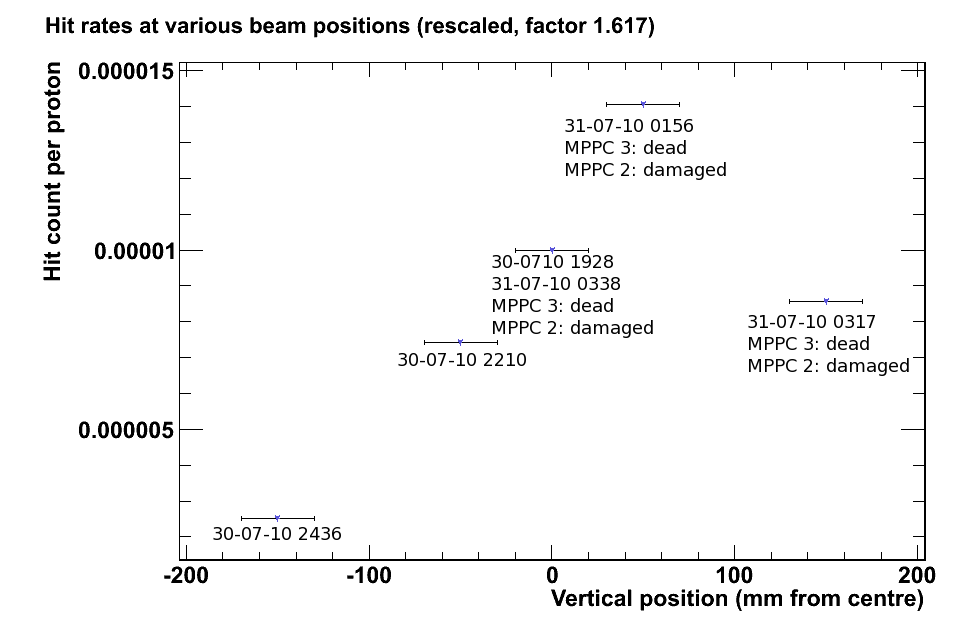
\includegraphics[width=.9\textwidth]{images/hit_rate_rescaled.png}
  \caption{Charged particle flux at a variety of vertical positions, 50~cm from the end of the MTS, at MuSIC. The note below each point indicates when the data was taken, the three right-most points have been rescaled (using the ratio of the 0~mm values) to account for the broken MPPCs (as noted). Measurement was taken using a \( 380\times30\times8 \)~mm scintillator mounted on aluminium support struts.}
  \label{fig:1D_hit_rate_rescaled}
\end{figure}

\begin{figure}[hptb]
  \centering
    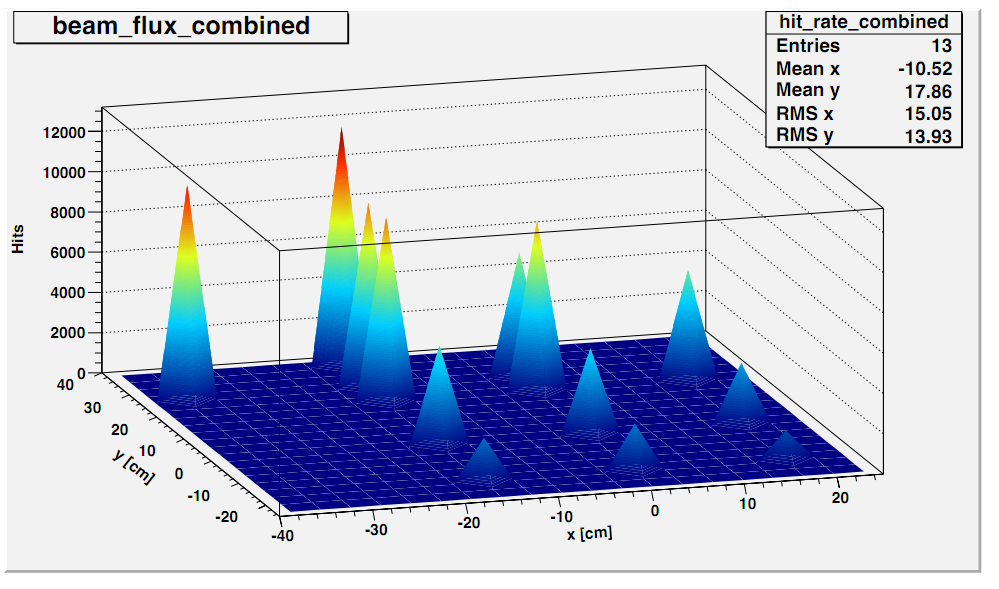
\includegraphics[width=.9\textwidth]{images/2D_hit_rate_dist.png}
  \caption{The charged particle flux at 5~cm from the end of the beam-pipe, measured using a 7~cm diameter scintillator.}
  \label{fig:2D_hit_rate_dist}
\end{figure}


% chapter charged_particle_flux (end)
%%%%%%%%%%%%%%%%%%%%%%%%%%%%%%%%%%%%%%%%%%%%%%%%%%%
\chapter{Muon Lifetime} % (fold)
\label{sec:muon_lifetime}
% TODO: Measurements:: Muon Lifetime: write me
% TODO: Measurements:: Muon Lifetime: cover set up
% TODO: Measurements:: Muon Lifetime: cover daq
% TODO: Measurements:: Muon Lifetime: cover first data set vs second
\begin{figure}[hptb]
  \centering
    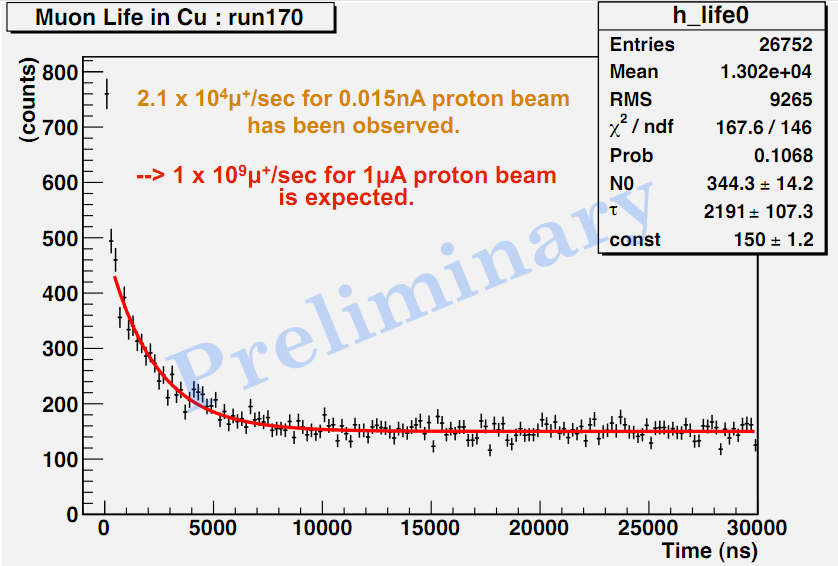
\includegraphics[width=.9\textwidth]{images/muon_decay_feb.png}
    % TODO Add PDG muon lifetime
  \caption{First measurement of the muon lifetime at MuSIC. A single exponential is used for the fit and the lifetime measured is compatible with the global measurement (PDG MUON LIFETIME~\cite{pdg for muons}).  } 
  \label{fig:3_measurements_images_muon_decay_feb}
\end{figure}

\begin{figure}[hptb]
  \centering
    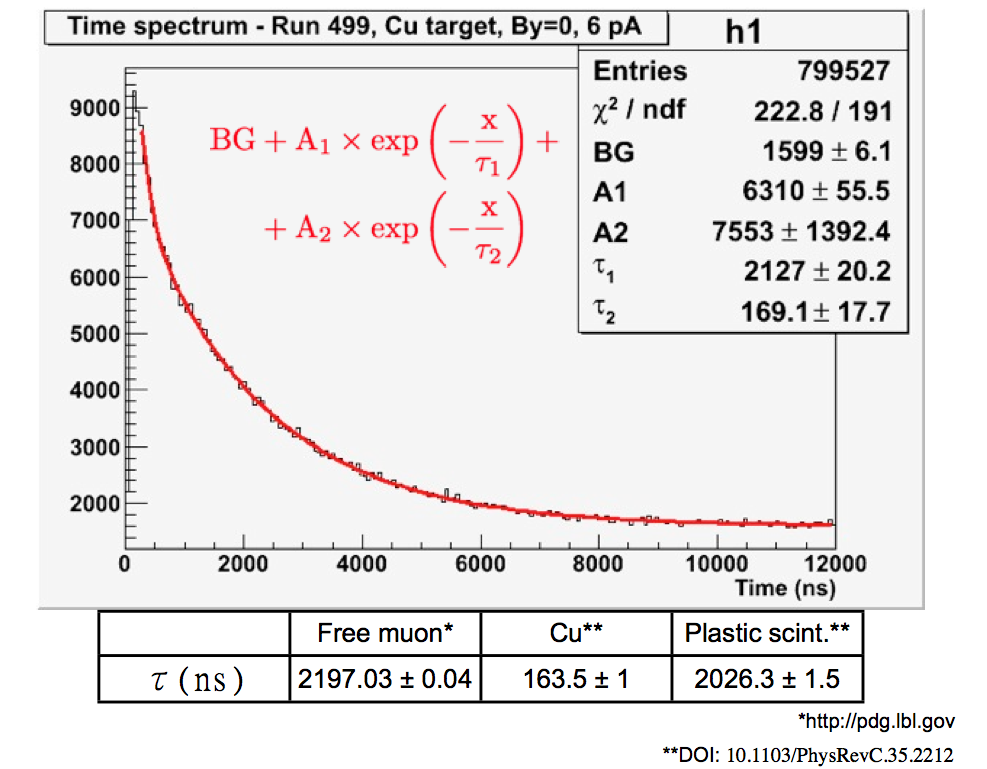
\includegraphics[width=.9\textwidth]{images/muon_decay.png}
  \caption{Second measurement of muon lifetime at MuSIC, made 19\( ^{th} \)--21\( ^{st} \)~July~2011. With the improved statistics a double exponential was used allowing an estimation of the \( \mu^{-} \) component to be made. This estimation is made by looking for muons stopping in the copper target. The muon lifetime is low but this is to be expected as there is a hidden component due to negative muons interacting with the scintillator and air~\cite{Muon lifetime in scintillator}.}
  \label{fig:3_measurements_images_muon_decay}
\end{figure}


% chapter muon_lifetime (end)
%%%%%%%%%%%%%%%%%%%%%%%%%%%%%%%%%%%%%%%%%%%%%%%%%%%
\chapter{Muon Momentum Spectrum} % (fold)
\label{sec:muon_momentum_spectrum}
% TODO: Measurements:: Muon Momentum Spectrum: write me
% TODO: Measurements:: Muon Momentum Spectrum: daq & set up 
% TODO: Measurements:: Muon Momentum Spectrum: noise
% TODO: Measurements:: Muon Momentum Spectrum: sensitve to
% TODO: Measurements:: Muon Momentum Spectrum: stopping targets

\section{Experimental Set Up} % (fold)
\label{sec:experimental_set_up}
To measure the momentum distribution of the muon beam two separate problems had to be solved: firstly how to count the muons produced and secondly how to determine their momentum. The first problem is addressed by looking for muon decays through timing data whilst the second is dealt with by using degraders and a thin stopping target to select specific momentums. 

\subsection{Detector} % (fold)
\label{sub:detector}
The detector consisted of an aluminium degrader who's thickness could be varied to select different momentum ranges, a thin (0.5~mm) upstream counter and a thicker (3.5~mm) downstream counter on either side of a 0.5~mm copper stopping target. A schematic of the detector can be seen in figure~\ref{fig:setup}. Based on simulation (section~\ref{sec:simulated_data}) we can predict the mean momentum of muons that decay for different degrader thicknesses, the momentum distributions for the muons that stop can be seen in figure~\ref{fig:stopped_muon_mom} whilst the initial muon momentum distribution is given in figure~\ref{fig:initial_muon_momentum}, the mean momentums are also tabulated in table~\ref{tab:stopped_muon_mom}.
\begin{figure}[htbp]
    \centering
        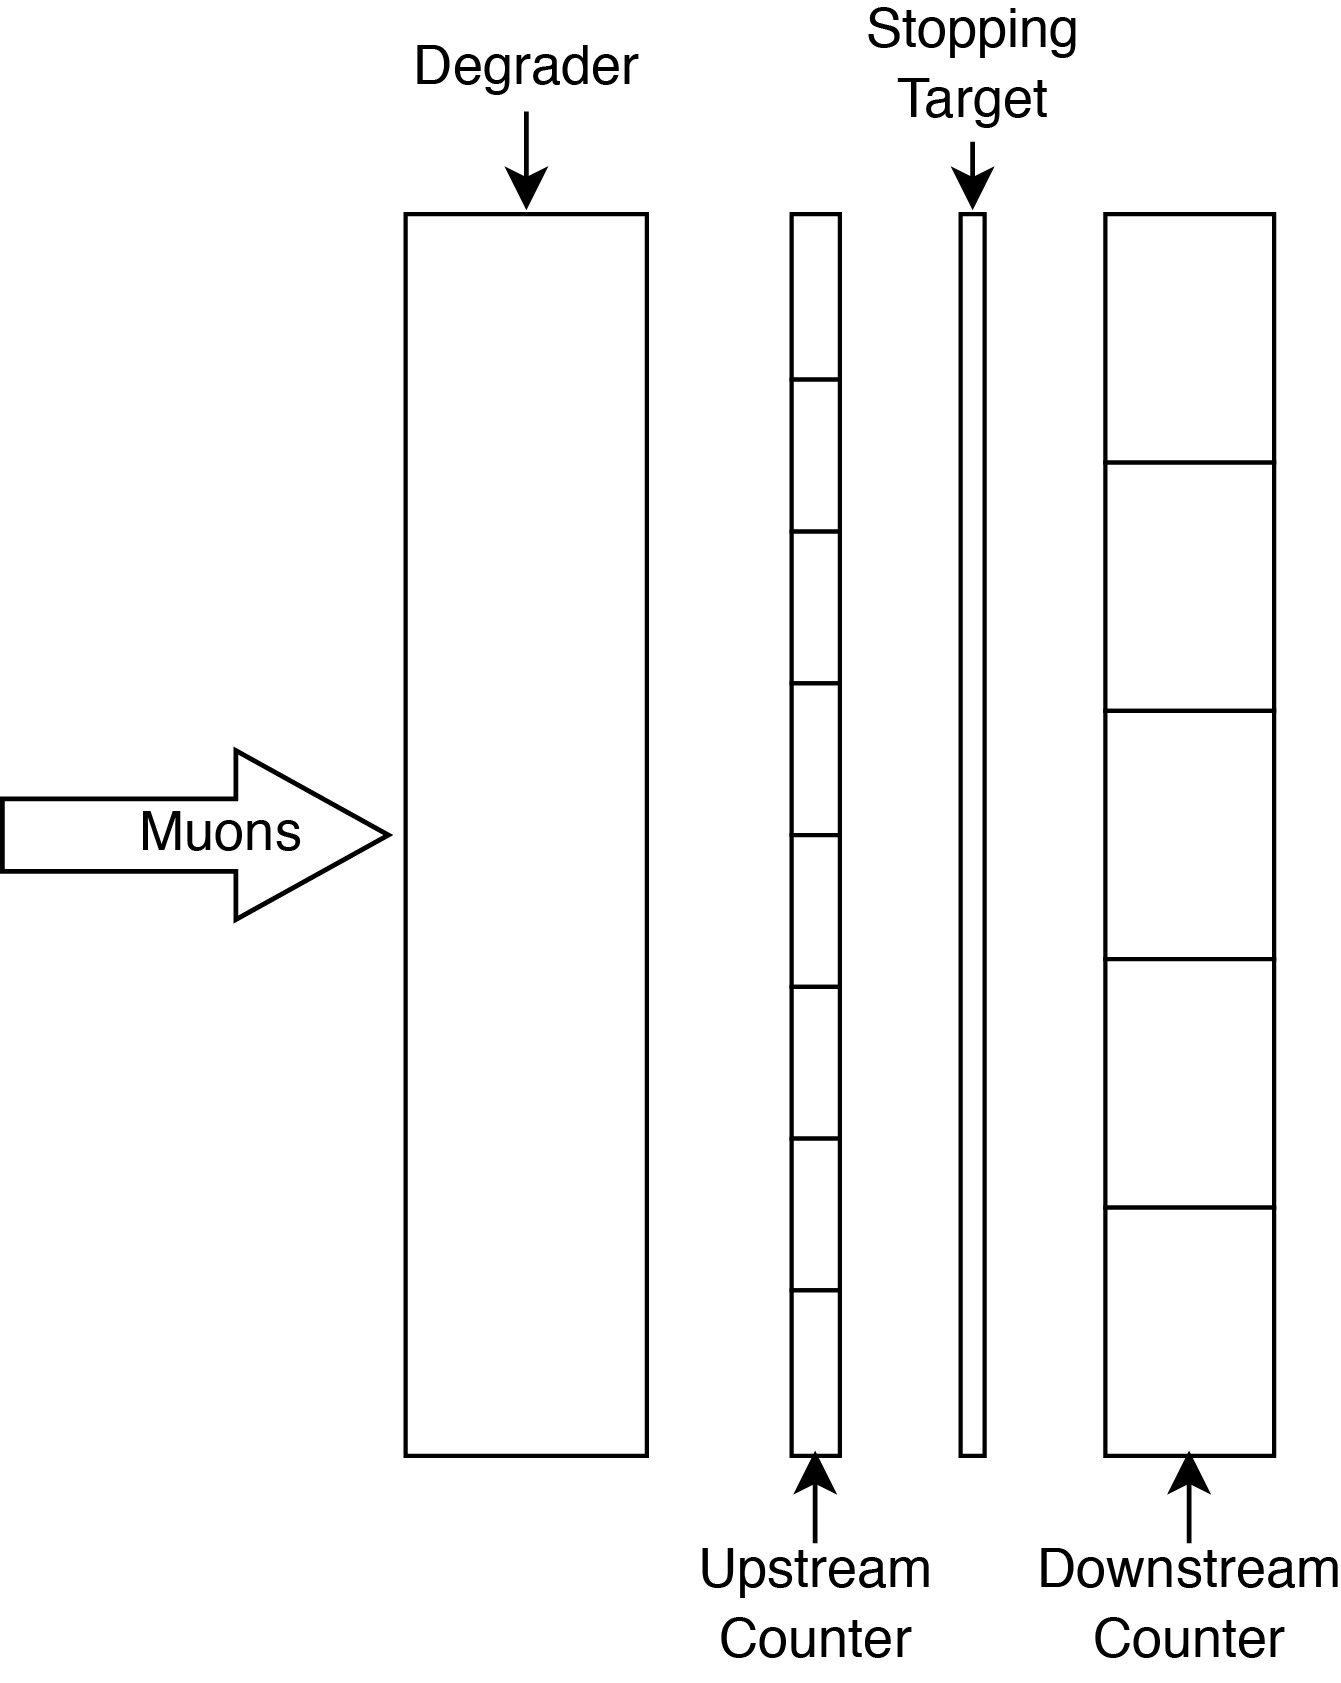
\includegraphics[scale=0.5]{images/Detector_setup.png}
    \caption{Experimental set up of the detector for MuSIC~5 (not to scale)}
    \label{fig:setup}
\end{figure}  
%
\begin{figure}[htbp]
    \centering
        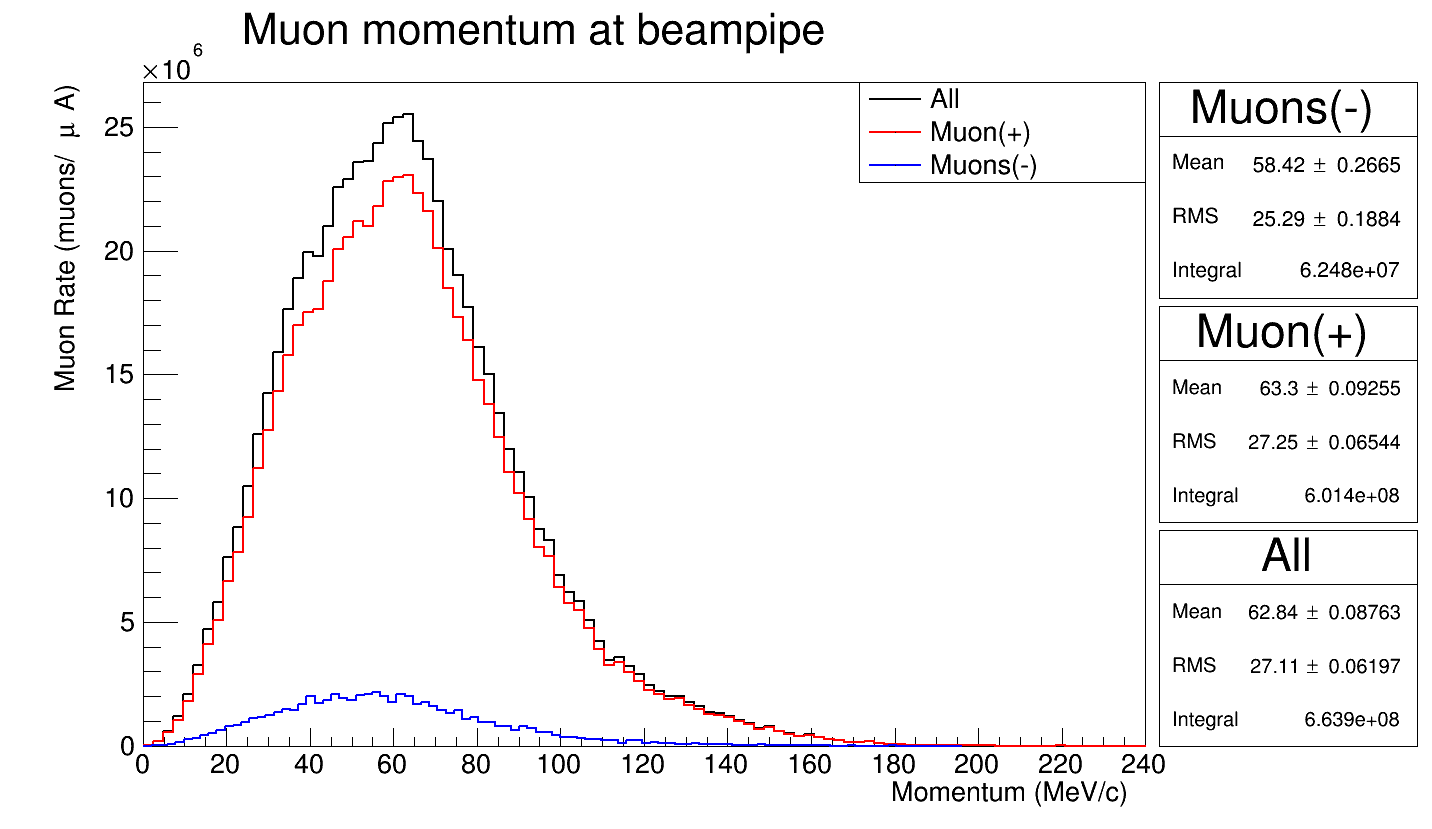
\includegraphics[width=\textwidth]{images/muon_momentum_at_beam_pipe_exit.png}
    \caption{The initial muon momentum at the exit of the beampipe as simulated by G4Beamline~\cite{G4BL} (G4BL). The muon rate has been normalised to \( 1\mu \)A of proton current which is the maximum available at the RCNP. Section~\ref{sub:g4bl_particle_production} for further details of the G4BL simulation.}
    \label{fig:initial_muon_momentum}
\end{figure}
%
\begin{figure}[htbp]
    \centering
        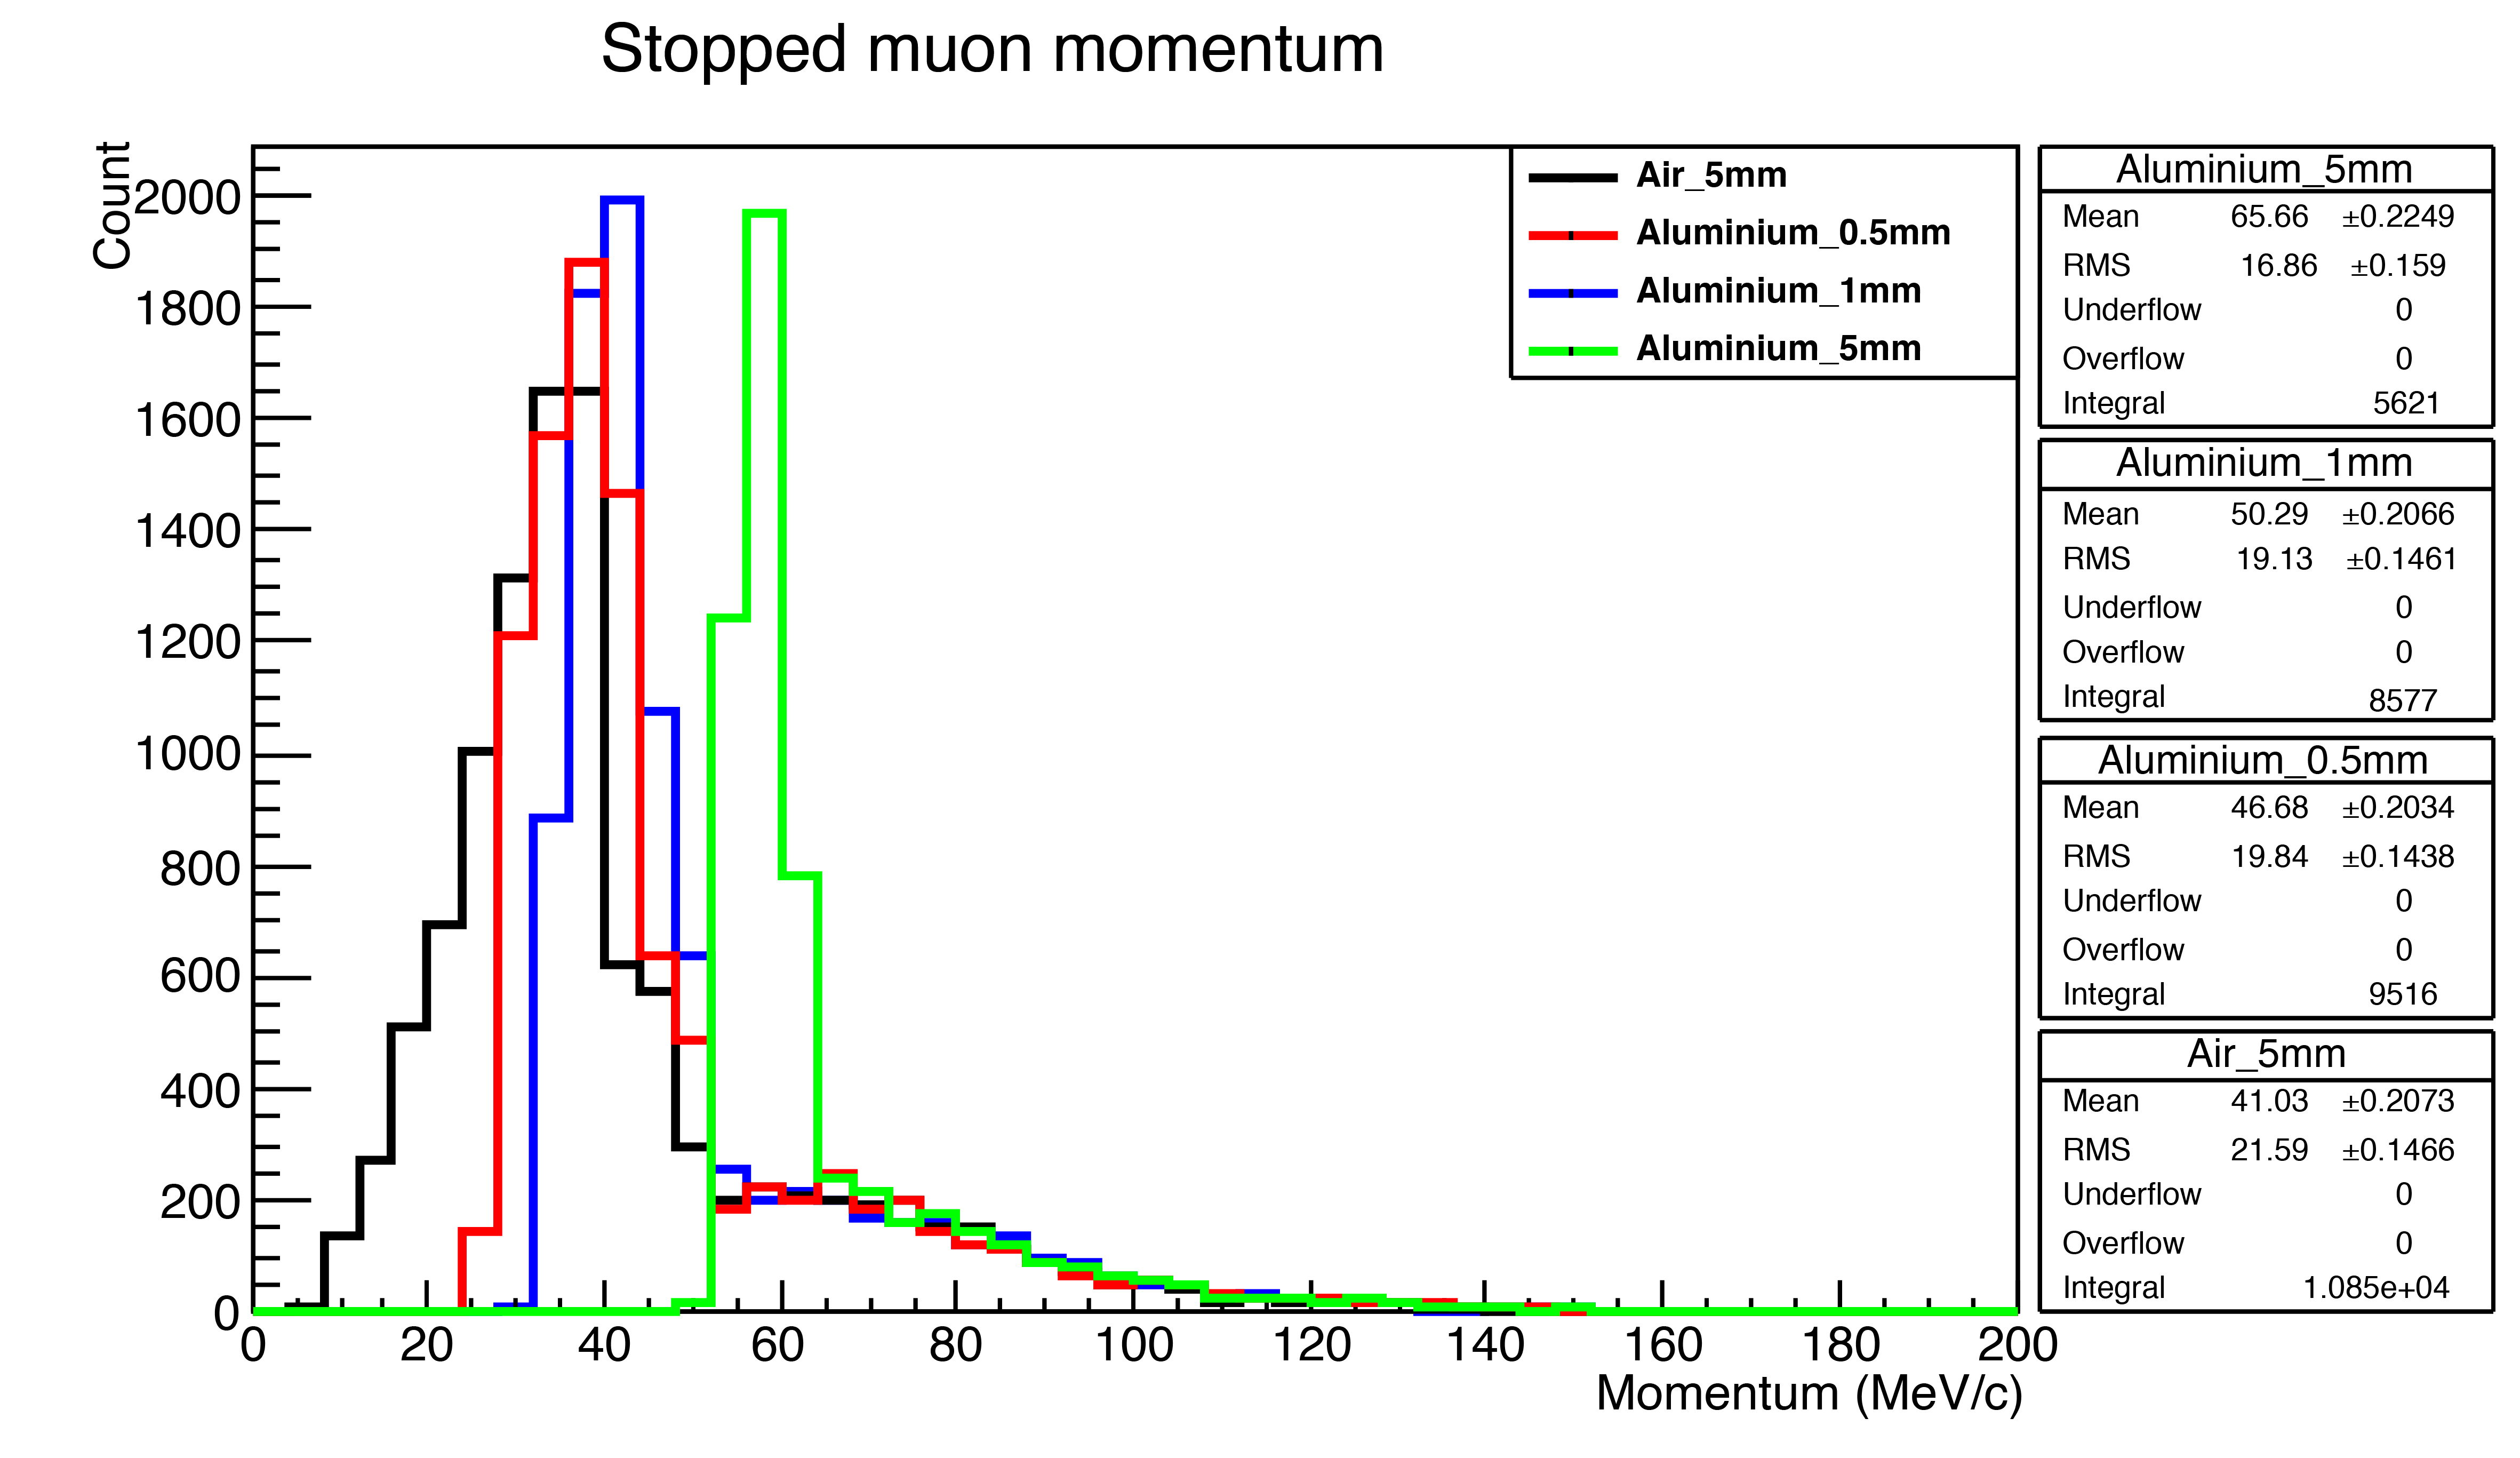
\includegraphics[width=\textwidth]{images/stopped_muon_momentum.png}
    \caption{Simulated momentum distributions for muons that decay between the up and downstream counters. 900~M initial protons were simulated with a range of aluminium degrader thicknesses. Stopped muons were those seen in the upstream counter that subsequently had a daughter electron seen in the downstream counter. This plot shows raw counts for the 900~M initial protons.}
    \label{fig:stopped_muon_mom}
\end{figure}
%
\begin{table}
    \begin{center}
    \begin{tabular}{r|r@{ $\pm$ }l|r@{ $\pm$ }l} % r@{ $\pm$ }l should align on \pm
        Degrader (mm) & \multicolumn{2}{|c|}{Mean (MeV/c)} & \multicolumn{2}{|c}{RMS (MeV/c)}\\
        \hline
        Air 5.0       & 41.03 & 0.21 & 21.59 & 0.15 \\
        Aluminium 0.5 & 46.68 & 0.20 & 19.84 & 0.14 \\
        Aluminium 1.0 & 50.29 & 0.21 & 19.13 & 0.15 \\
        Aluminium 5.0 & 65.66 & 0.22 & 16.86 & 0.16 \\
    \end{tabular}
    \end{center}
    \caption{Simulated mean momentums for decaying muons. 900~M initial protons}
    \label{tab:stopped_muon_mom}
\end{table}
%
The counters used were mylar wrapped scintillators with read-out performed by MPPCs mounted on either end of a wave length shifting fibre bounded along the long axis of the scintillator using optical cement. The signals from each pair of MPPCs are combined and amplified before being passed to the data acquisition system (DAQ) for processing.

% subsection detector (end)
\subsection{Data Acquisition} % (fold)
\label{sub:data_acquisition}
The Data Acquisition (DAQ) took two measurements: the time at which signals arrived from the MPPC and the strength of those signals. The timing measurements are of the primary concern for this analysis. The DAQ itself had 3 distinct stages: discrimination, trigger formation and readout.

MPPCs are inherently noisy devices and discrimination is required to separate signal due to scintillation events from the MPPC's noise. A voltage threshold was set which (when exceeded) created a digital signal. Two thresholds were used: a lower one for the upstream counter and a higher one for the downstream counter. The lower threshold for the, thinner, upstream counters enabled better detection of minimally ionising muons whilst the higher downstream threshold enabled better detection of the more ionising electrons produced by muon decay. 

Using the signals from the discriminator a trigger was created based on the signature of muonic decay: the anti-coincidence of the up and downstream counters. It was assumed that a muon that doesn't decay in the detector region will be seen in both counters within a very small window of time ($<$50~ns). The only other constraint on the formation of a trigger was that the system wasn't busy in which case the trigger couldn't be accepted.

The trigger, once formed, signalled the start of readout. There were 3 modules to be read out via VMEbus (VME): a charge to Digital Converter (QDC), a scaler and a Multi-hit Time to Digital Converter (MTDC) which is of primary concern for this analysis. The MTDC recorded all signals  within a 20\mus{} period following the trigger that passed discrimination and that were anti-coincident with the other counter. Using a MTDC ensured that even if some beam remnant or dark event created a signal then the real signal would also be recorded and determined with background removal. The channel assignment used for the MTDC can be seen in table~\ref{tab:mtdc_ch}. To increase the accuracy of the MTDC the trigger time is recorded on a seperate channel called `TDC0'.
\begin{table}
    \begin{center}
    \begin{tabular}{c|c|c}
        Channel & Signal & Notes\\
        \hline
        0  & TDC0 & Time at which the trigger was formed \\
        \hline
        1  & U1   & \multirow{8}{*}{Upstream Counter}\\
        2  & U2   & \\
        3  & U3   & \\
        4  & U4   & \\
        5  & U5   & \\
        6  & U6   & \\
        7  & U7   & \\
        8  & U8   & \\
        \hline
        9  & D1   & \multirow{5}{*}{Downstream counter}\\
        10 & D2   & \\
        11 & D3   & \\
        12 & D4   & \\
        13 & D5   & \\
        \hline
        14 & Ge1  & \multirow{2}{*}{Germanium counter (not used in this analysis)}\\
        15 & Ge2  & \\
    \end{tabular}
    \end{center}
    \caption{Channel assignment for the MTDC. QDC channel assignment follows the same scheme but has no entry for channel 0 (as TDC 0 will be one of the upstream counters by design).}
    \label{tab:mtdc_ch}
\end{table}

The scaler was used to record system diagnostics (e.g. the trigger rate) by polling the scaler regularly during each run. The QDC recorded the strength of the trigging signal by integrating its charge over 100~ns. This information has not be incorporated into the current analysis but may be used in later analysis, for example to apply more stringent energy cuts at trigger time or for selection of regions of interest. The QDC had the same channel assignment as the TDC but without the germanium detector (as it had its own analogue to digital converter) and TDC0 (which was a digital signal).
\begin{table}
    \centering
    \begin{tabular}{c|c|l}
        Channel & Signal & Notes\\
        \hline
        0 & SEC & Measure of the proton current\\
        1 & Trigger & number of t0's\\
        2 & U and $\overline{\text{D}}$ & count of potential triggers\\
        3 & U & Upstream only\\
        4 & D & Downstream only\\
        5 & Scint & -\\
        6 & unused & -\\
        7 & clk & Record of time passed\\
    \end{tabular}
    \caption{Table of scaler channels and their designation}
    \label{tab:scaler_chs}
\end{table}
\section{Run Data} % (fold)
\label{sec:run_data}
As figure~\ref{fig:analysis_flow_diagrm} shows there are 5 stages in preparing the experimental data for analysis (receipt of the data from MIDAS, de-serialisation, calibration, restructuring and histogramming). These will will be explained in more detail in the following sub-sections but the general process will be discussed here. The first stage is the receipt of data from the DAQ via MIDAS, this creates files of raw data which has to be de-serialised in the next stage before having calibration applied to it. The final stages are to restructure the data according to channel and then create histograms of the TDC values ready for analysis. 

These processes are split across 4 programs: MIDAS; mu\_analysis and mid2root\_converter (which act on .root and .mid MIDAS files respectively); and finally tdc\_file.py which is a python script for creating the TDC histograms.

For the analysis 6 runs were chosen, all using the 0.5~mm copper stopping target. For 5 of the runs an aluminium degrader was used. The run information is summarised in table~\ref{tab:run_summary}.
\begin{table}
	\begin{center}
	\begin{tabular}{c|c|c|c}
		Run ID & Time (sec) & Current (nA) & Degrader (mm) \\
		\hline
		448    & 9,221      & 1.534E-02    & 0.0   \\
		451    & 1,001      & 1.546E-02    & 0.5   \\
		452    & 4,924      & 1.313E-02    & 0.5   \\
		455    & 6,307      & 1.332E-02    & 1.0   \\
		458    & 5,144      & 1.363E-02    & 5.0   \\
		459    & 2,452      & 1.238E-02    & 5.0   \\
	\end{tabular}
	\end{center}
	\caption{Summary of the runs selected for this analysis. The degrader used aluminium and the stopping target 0.5~mm copper.}
	\label{tab:run_summary}
\end{table} 
\subsection{Data from MIDAS} % (fold)
\label{sub:data_from_midas}
MIDAS is `a general purpose data acquisition system for small and medium scale experiments'~\cite{ritt2012midas} and is the primary interface to the DAQ via VME. 

MIDAS stored the raw data from each run as a single file either in its own binary xml format (.mid files) or in ROOT~\cite{Brun199781} format (.root). Data was read from the VME crate in two asynchronous modes: `Trigger' and `Scaler' each corresponded to a separate tree structure in the resulting file. The majority of the time the system operated in trigger-mode: whenever a trigger was formed the controlling PC was informed and once the data had been gathered readout of the MTDC and QDC occurred via the VME. Scaler mode occurred at regular intervals and consisted of reading the diagnostics data gathered by the scaler, this did not reset the module which continued to accumulate data. 

Each tree contained a branch per module being read, the trigger tree also had also branch for errors (named `ERR'). The branches all had the same structure: an integer that recorded the number of values read and an array of integers containing those values. For the scaler and QDC modules the number of values read out was the same for every trigger as both had a fixed number of channels and took one measurement on each. The MTDC had a variable number of values to read out as it could record multiple hits on each channel.
% subsubsection data_from_midas (end)
\subsection{De-Serialisation} % (fold)
\label{sub:de_serialisation}
The first raw data from MIDAS for the MTDC and QDC were serialised and mangled with the channel number this means that they require processing before the real values can be extracted. Below are brief summaries of the algorithms used to de-serialise the MTDC data (listing~\ref{lst:mtdc_algo}), for full listings, including de-serialisation methods for QDC, see appendix~\ref{app:deserialisation}.
%
\begin{listing}[htbp]
    \begin{minted}[gobble=4]{c++}
    tdc_value      =  raw_val & 0x001f ffff
    tdc_channel    = (raw_val & 0x03e0 0000) >> 21
    tdc_valid_read = (raw_val & 0xf800 0000) == 0x0
    \end{minted}
    \caption{Method for de-serialising CAEN V1290N~\cite{CAENV1290N} data}
    \label{lst:mtdc_algo}
\end{listing}
% subsection de_serialisation (end)
\subsection{Calibration} % (fold)
\label{sub:calibration}
The MTDC has a stated least significant bit resolution of $\sim$25~ps with a 21 bits of data per value, this gives a maximum value of 52\mus{}. Conversion from the stored value to real, trigger aligned, time is done using the formula:
\begin{align}\label{equ:tdc_calibration}
    t'   &= 0.024414(t - \text{TDC}0)
\end{align}
where $t'$ is the calibrated time, $t$ is the de-serialised MTDC value and TDC$0$ is the de-serialised trigger time. The value $0.024414$ is the calibration co-efficient as determined in Tran Nam's work~\cite{timecalibNam2012}
% subsection calibration (end)
\subsection{Restructure} % (fold)
\label{sub:restructure}
In order for the MIDAS data to be easily manipulated it was restructured. The initial format was a simple structure of one branch for each module (i.e. one for MTDC one for the QDC and a final one for errors). A second tree was used to store the scaler values. Each branch had a leaf for the number of values and a leaf with the array of values.

In the restructured file each channel is a branch of a tree with the following leaves: QDC, TDC0, nHITS, TDC[nHITS]. The QDC value is self-explanatory, TDC0 was the trigger time, nHITS was the number of entries recorded by the MTDC for that channel and TDC was an array of the values. The error data was ignored as was the scaler tree as these can be read from the original file if needed and neither was required for de-serialisation or calibration.
% subsection restructure (end)
\subsection{Histogramming} % (fold)
\label{sub:Histogramming}
Once the data has been restructured it is trivial to create a histogram of the TDC data for each channel which forms the basis of the later analysis. A basic bin width of 1~ns was used and a range from 0 to 20\mus. A time of 0 was used for the lowest bin as, although the data window began at 50~ns, the MTDC recorded data as a sliding window so some values prior to the trigger were also recorded. All the histograms for (i.e. for all channels for all runs) were saved in the same root file.
% subsection histogramming (end)
% section run_data (end)
%%%%%%%%%%%%%%%%%%%%%%%%%%%%%%%%%%%%%%%%%%%%%%%%%%%%%%%%%%%%%%%%%%%%%%%%%%%%%%
\section{Secondary calculations} % (fold)
\label{sec:secondary_calculations}
There are two secondary calculations that need to be performed to calculate the muon yield. These are the acceptance, the fraction of the total beam we can expect to detect, and the dead time, a measure of how much of the time the detector is unable to process new data due to being busy.
\subsection{Acceptance} % (fold)
\label{sub:acceptance}
To calculate the acceptance the ratio of initial muons to muons that passed a `trigger' cut was calculated. This is done by counting the number of muons in simulated G4BL output (section~\ref{sub:g4bl_particle_production}) and then using a macro similar to that used to digitise the simulation output (section~\ref{sub:digitisation_histogramming}) to mimic the triggering process.

The main difference between the acceptance macro (appendix~\ref{appsub:acceptance}) and the digitisation macro (appendix~\ref{appsub:digitisation_macro}) were in the cuts applied to select the particles. Rather than any possible parent particle in the upstream detector only muons are selected, similarly, in the downstream detector only electrons who had a parent muon are selected. A final requirement is that the time difference between muon and electron is greater than 50~ns.

The acceptance is then the ratio of muon/electron pairs to the initial number of muons:
\begin{align}
    \text{Acceptance} &= \frac{\text{Decay muons}}{\text{Initial Muons}} \label{equ:acceptance}
\end{align}
It is worth noting that given the above definition and method the acceptance changes due to the thickness and type of degrader used. Obviously a degrader that removed the majority of the muons from the beam will have a smaller acceptance as a smaller fraction of the beam will have survived to be detected. The results of the acceptance calculations are given in table~\ref{tab:acceptance}, the macro used can be seen in appendix~\ref{appsub:acceptance}.
\begin{table}
    \begin{center}
    \begin{tabular}{c| r@{ $\pm$ }l | r@{ $\pm$ }l | r@{ $\pm$ }l | r@{ $\pm$ }l }
        Degrader (mm) & \multicolumn{2}{|c}{Count (no cut)} &
                        \multicolumn{2}{|c}{Count ($\Delta t>50$~ns)} &
                        \multicolumn{2}{|c}{Initial Muons} &
                        \multicolumn{2}{|c}{Acceptance (\%)}\\
        \hline
              Air 5.0 & 6330 & 80 & 4540 & 67.4 & 95719 & 309.4 & 4.7 & 0.1\\
        Aluminium 0.5 & 5636 & 75 & 3999 & 63.2 & 95719 & 309.4 & 4.2 & 0.1\\
        Aluminium 1.0 & 5222 & 72 & 3689 & 60.7 & 95719 & 309.4 & 3.9 & 0.1\\
        Aluminium 5.0 & 3632 & 60 & 2472 & 49.7 & 95719 & 309.4 & 2.6 & 0.1\\
        
    \end{tabular}
    \end{center}
    \caption{The variance of acceptance with degrader thickness. In the final acceptance a cut on $\Delta t$ requiring it to be $>$50~ns was used to account for the anti-coincidence of the downstream counter. The number of initial muons is from the G4Beamline simulation.}
    \label{tab:acceptance}
\end{table}
% subsection acceptance (end)
\subsection{Dead time} % (fold)
\label{sub:dead_time}
The calculation of the dead time is unlike that of the acceptance as it was calculated based on the real data rather than simulation. Using the scaler it is possible to estimate how much of the time the DAQ was busy and hence what percentage of data was missed. 

As was stated in section~\ref{sub:data_acquisition} the scaler was used to record diagnostics on the DAQ. To calculate the dead time only two are needed, the trigger count and the potential trigger count which can be used to calculate the dead time thus:
\begin{align}
    D = \frac{\text{Potential Triggers}}{\text{Good Triggers}}
\end{align}
Where potential triggers are considered any anti-coincidence of the up without the downstream counter and a good trigger is one in which this occurs without the system being busy. The results for are given in table~\ref{tab:dead_time}. Obviously, the dead time is not used in the yield calculations using the simulated data.
\begin{table}
    \begin{center}
    \begin{tabular}{c|c|c|r@{ $\pm$ }l|r@{ $\pm$ }l|r@{ $\pm$ }l }
        Run & Degrader (mm of Al) & Run time (s) &
                              \multicolumn{2}{|c}{Good Triggers} &      
                              \multicolumn{2}{|c}{Potential Triggers} &
                              \multicolumn{2}{|c}{Dead time (\%)} \\
        \hline
        448 & 0.0 & 9221 & 9652965 & 3106 & 15678757 & 3959 & 61.57 & 0.03 \\
        451 & 0.5 & 1001 &  767321 & 875  &  1070366 & 1034 & 71.69 & 0.11 \\
        452 & 0.5 & 4944 & 3459886 & 1860 &  4667767 & 2160 & 74.12 & 0.05 \\
        455 & 1.0 & 6307 & 4090246 & 2022 &  5372409 & 2317 & 76.13 & 0.05 \\
        458 & 5.0 & 5144 & 2049077 & 1431 &  2454952 & 1566 & 83.47 & 0.08 \\
        459 & 5.0 & 2452 &  915314 & 956  &  1077534 & 1038 & 84.95 & 0.12 \\
    \end{tabular}
    \end{center}
    \caption{Dead time for each run along with the number of potential and good triggers. Run time is included to show the origin of the different counts.}
    \label{tab:dead_time}
\end{table}
% subsection dead_time (end)
\subsection{Gain stability} % (fold)
\label{sub:gain_stability}
In order to better understand possible sources of systematics in the experiment the total trigger rate for each run was plotted over time. The gain stability should then be proportional to this trigger rate, giving a measure of how well the detector was working and highlighting any possible problems in the run. To plot this value the events produced in a run were divided into 10 sections, each containing an equal number of events. Using the values recorded by the scaler the length of each section in seconds could be determined (channel 7, see table~\ref{tab:scaler_chs}) as could the number of triggers seen in that section (channel 1). The results are plotted in figure~\ref{fig:gain_stability}, note that as the degrader thickness is increased the fit value decreases which is consistent with fewer particles reaching the detector. Full listings for plotting the gain stability can be found in appendix~\ref{appsub:gain_stability}.
%
\begin{figure}[htbp]
    \centering
        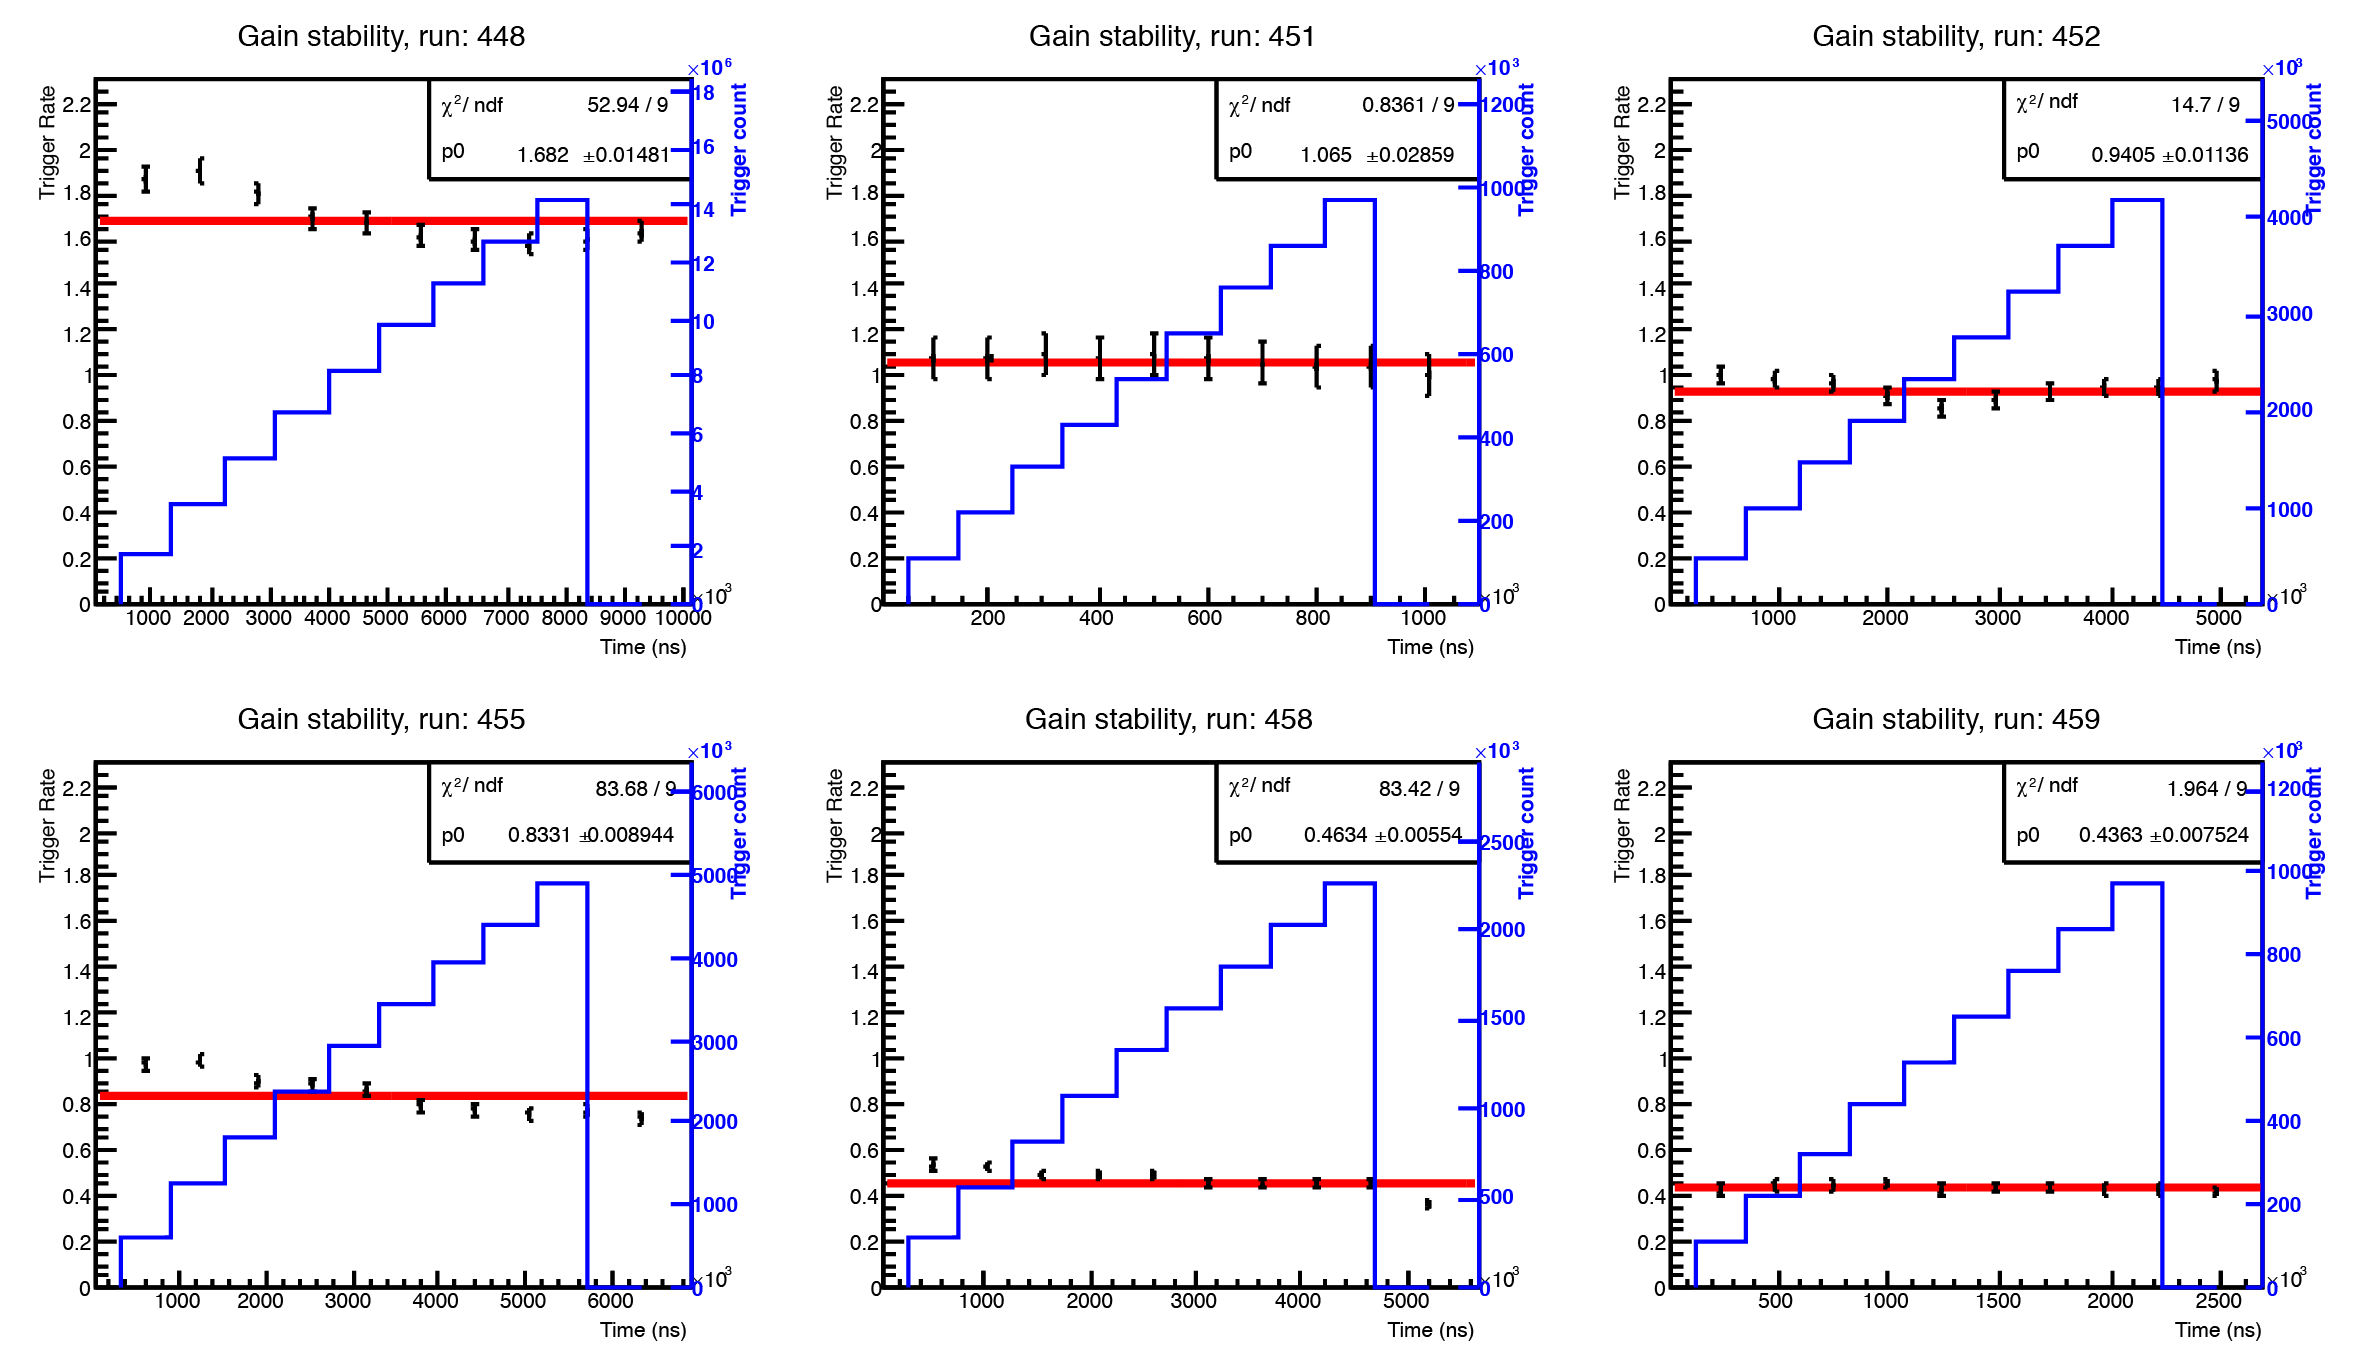
\includegraphics[width=\textwidth]{images/gain_stability.png}
    \caption{Gain stability for each run, the black lines indicate the gain stability for that period of time (each $\sim^1/_{10}^{\text{th}}$s of the run) whilst the blue histogram plots the cumulative number of triggers. The gain stability has bit fitted with an order 0 polynomial who's parameters are given.}
    \label{fig:gain_stability}
\end{figure}
%
\begin{table}
    \begin{center}
        \begin{threeparttable}
            \begin{tabular}{c|c|c|c|r@{ $\pm$ }l}
                Run & Al degrader thickness (mm) & $\chi^2$ 
                                                 & N.D.F. \tnote{a}
                                                 & \multicolumn{2}{|c}{Gain} \\
                \hline
                448  &  0.0  &  52.94   &  9  &  1.682  &  0.015  \\
                451  &  0.5  &  0.8361  &  9  &  1.065  &  0.029  \\
                452  &  0.5  &  14.7    &  9  &  0.940  &  0.011  \\
                455  &  1.0  &  83.68   &  9  &  0.8331 &  0.0089 \\
                458  &  5.0  &  83.41   &  9  &  0.4634 &  0.0055 \\
                459  &  5.0  &  1.964   &  9  &  0.4363 &  0.0075 \\
            \end{tabular}
            \caption{Gains as determined by the fits to the gain stability in figure~\ref{fig:gain_stability}.}
            \begin{tablenotes}
                \item [a] Number of Degrees of Freedom
            \end{tablenotes}
            \label{tab:gain_stability_paramters}
        \end{threeparttable}
    \end{center}
\end{table}

% subsection gain_stability (end)
% section secondary_calculations (end)
%%%%%%%%%%%%%%%%%%%%%%%%%%%%%%%%%%%%%%%%%%%%%%%%%%%%%%%%%%%%%%%%%%%%%%%%%%%%%%
\section{Fitting And Integration} % (fold)
\label{sec:fitting_and_integration}
This section won't follow the figure~\ref{fig:analysis_flow_diagrm} stages too closely as they are heavily entwined, instead the algorithm will be broken into two sections: the theory (section~\ref{sub:the_theory}) and the implementation (section~\ref{sub:the_implementation}).

\subsection{The theory} % (fold)
\label{sub:the_theory}
Once both the real and simulated data has been processed and put into histograms they can be treated identically. In order measure the number of decays the histograms are fitted with the function 
\begin{align}
    P(signal) &= N_{b} + N_{f}e^{-t / \tau_{f}} + N_{c} e^{-t / \tau_{c}} \label{equ:fit}
\end{align}
Where $N_{b}$ is a flat modelling of the background; $N_{f}$ and $\tau_{f}$ are the contribution of the free muon part and the free muon lifetime respectively; and $N_{c}$ and $\tau_{c}$ are the muonic-copper contribution and lifetime. Once the histogram has been fitted with equation~\ref{equ:fit} integrating either exponential portion of it and dividing by the bin width gives the number of muon decays corresponding to that mode. Similarly the total number of muons is given by the sum of the two integrals:
\begin{align}
    N_{\mu} &= \frac{1}{B} \int_{l}^{u}\left(N_{f}e^{-t / \tau_{f}} + N_{c} e^{-t / \tau_{c}} \right) \label{equ:sum_exp_parts}
\end{align}
where $N_{\mu}$ is the total number of muon decays in the histogram and $l$ and $u$ are the lower and upper bounds of the fit respectively. 

Obviously this is not a perfect analysis, as can be see from the histograms for simulation and data (figure~\ref{fig:example_fits_data_and_sim}) there are large differences between the backgrounds. As discussed above the majority of the background can be modelled as a flat distribution and hence subtracted there are, though, physics backgrounds that can mimic the expected signal of a muon decaying. The primary source of this will likely be pions luckily these backgrounds are very small as its lifetime is much shorter (26~ns compared to 2.2\mus{} for the muon) these short lifetimes will unlikely trigger due to the anti-coincidence.

% subsection the_theory (end)
\subsection{The implementation} % (fold)
\label{sub:the_implementation}
The implementation of the above algorithm is done using pyROOT~\cite{lavrijsenpyroot} which is a python wrapper for ROOT~\cite{Brun199781}. Python is a preferable language to C++ for complex analysis as it is generally less verbose (allowing more rapid development and fewer bugs) as well as incorporating more powerful data structures (such as dictionaries) into the core language. Being a loosely typed language python can handle mixed-type objects which means that all the data for run can be kept in a single structure. For concrete listings of each stage from figure~\ref{fig:analysis_flow_diagrm} see appendix~\ref{app:fitting_and_integration}.

There are 8 parameters that need to be set before the fit can proceed these are shown in table~\ref{tab:typical_fit_values} along with their typical initial values. There are two broad groups of parameter: `fit settings' which relate to the bounds on the fitting method and the `initial parameter values' which determine what values the fit uses as start points for its approximations. The fit settings primarily affect how good a fit is achieved whilst the initial parameter values are mainly chosen to ensure that there are no degeneracies in the fit. 

\begin{table}
    \begin{center}
	    \begin{threeparttable}
		    \begin{tabular}{c | c | c }
		        Type & Parameter   & Value \\
		        \hline
		        \multirow{3}{*}{Fit Settings} & Bin width   & 75~ns \\
		                                      & Lower bound & 50~ns \\
		                                      & Upper bound & 20\mus \\
		        \hline
		        \multirow{3}{*}{Initial fit parameters} 
		                    & $N_{b}$     & $^1/_{10} \times$ maximum bin value \\
		                    & $N_{c}$     & Maximum bin value\\
		                    & $N_{f}$     & $^1/_{2} \times$ maximum bin value\\
		                    & $\tau_{c}$  & 163.5~ns $\pm$ 1~ns\\
		                    & $\tau_{f}$  & $\sim$2\mus\tnote{a}\\
		    \end{tabular}
		    \caption{Typical values for the fit parameters. \textbf{NB} that the copper value is often constrained as it is well know, the free muon lifetime is not well known as it is dependant on the combination of the muon lifetime in air, scintillator and as a free particle.}
		    \begin{tablenotes}
		        \item [a] The canonical free muon lifetime is 2.1969811$\pm$0.0000022\mus~\cite{Beringer2012}, see text for why this value is not fixed.
		    \end{tablenotes}
		    \label{tab:typical_fit_values}
	    \end{threeparttable}
    \end{center}
\end{table}
%
\begin{figure}[htbp]
    \centering
        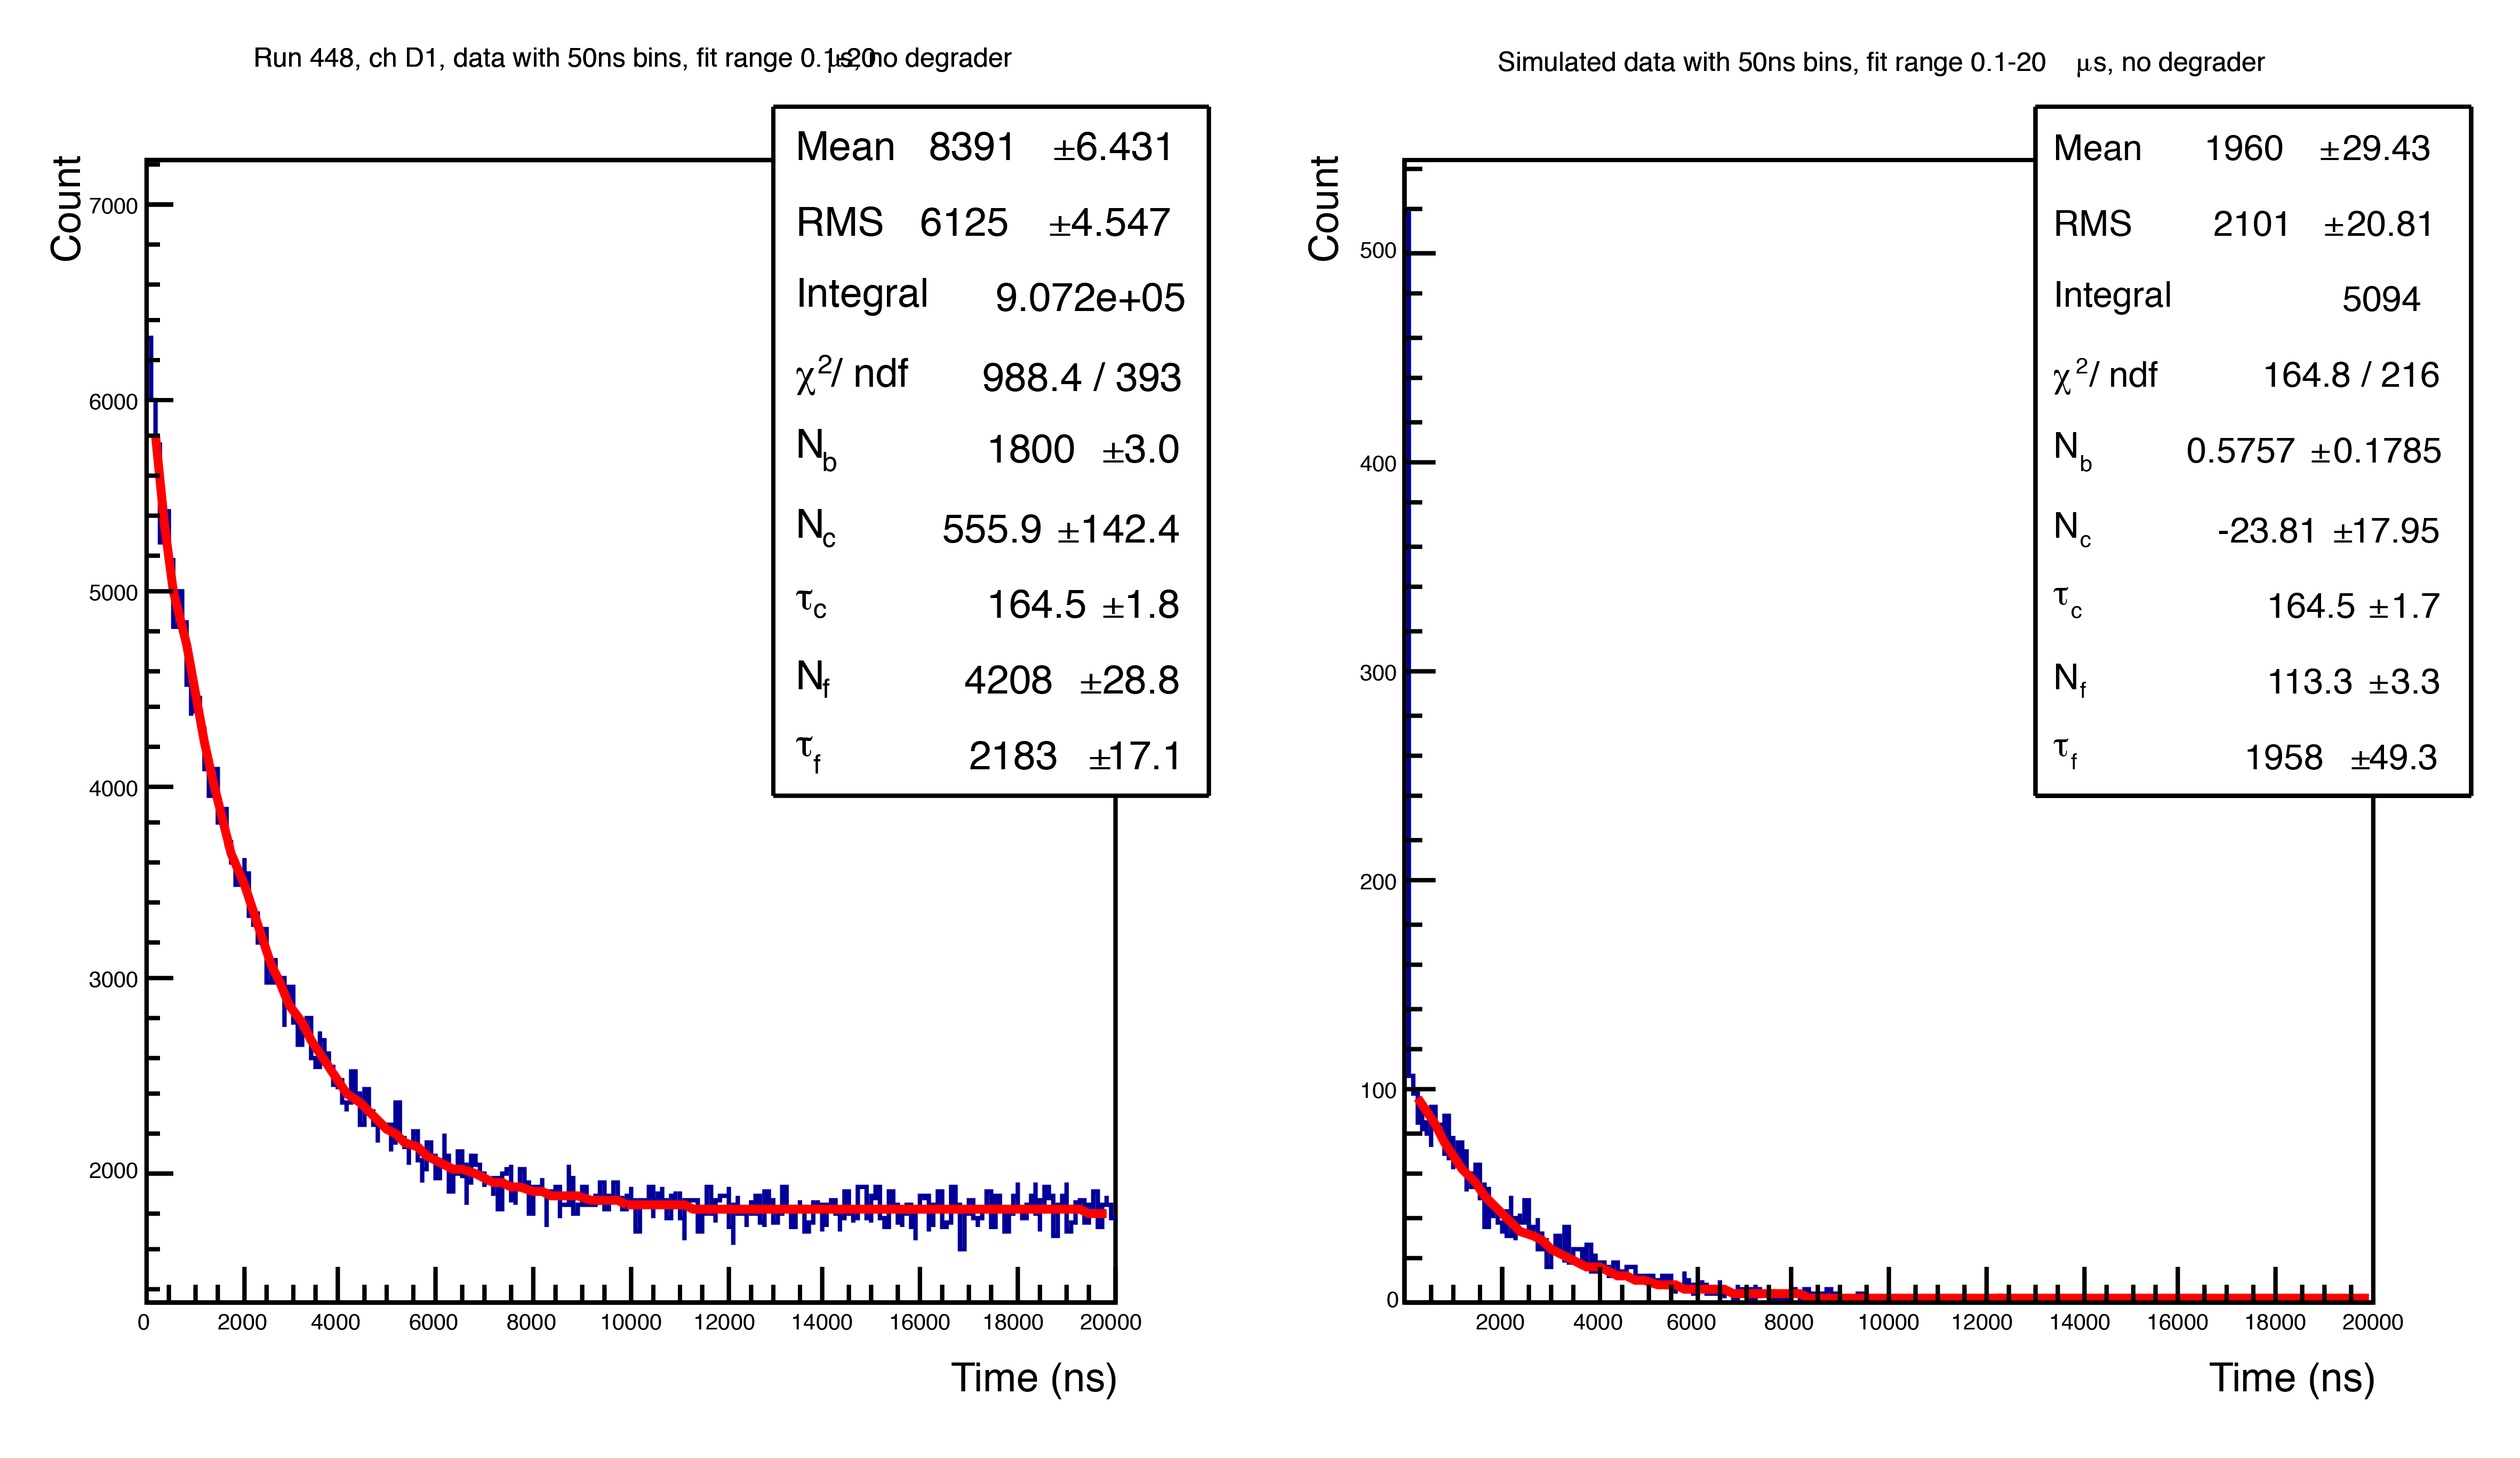
\includegraphics[width=\textwidth]{images/example_fits_data_and_sim.png}
    \caption{Example of typical histograms for both simulation and data. Each has been fitted with equation~\ref{equ:fit} using initial fit settings matching those in table~\ref{tab:typical_fit_values}. The run used was 448, channel D1, i.e. no degrader, and simulation was for air only.}
    \label{fig:example_fits_data_and_sim}
\end{figure}

\begin{figure}[htbp]
    \centering
        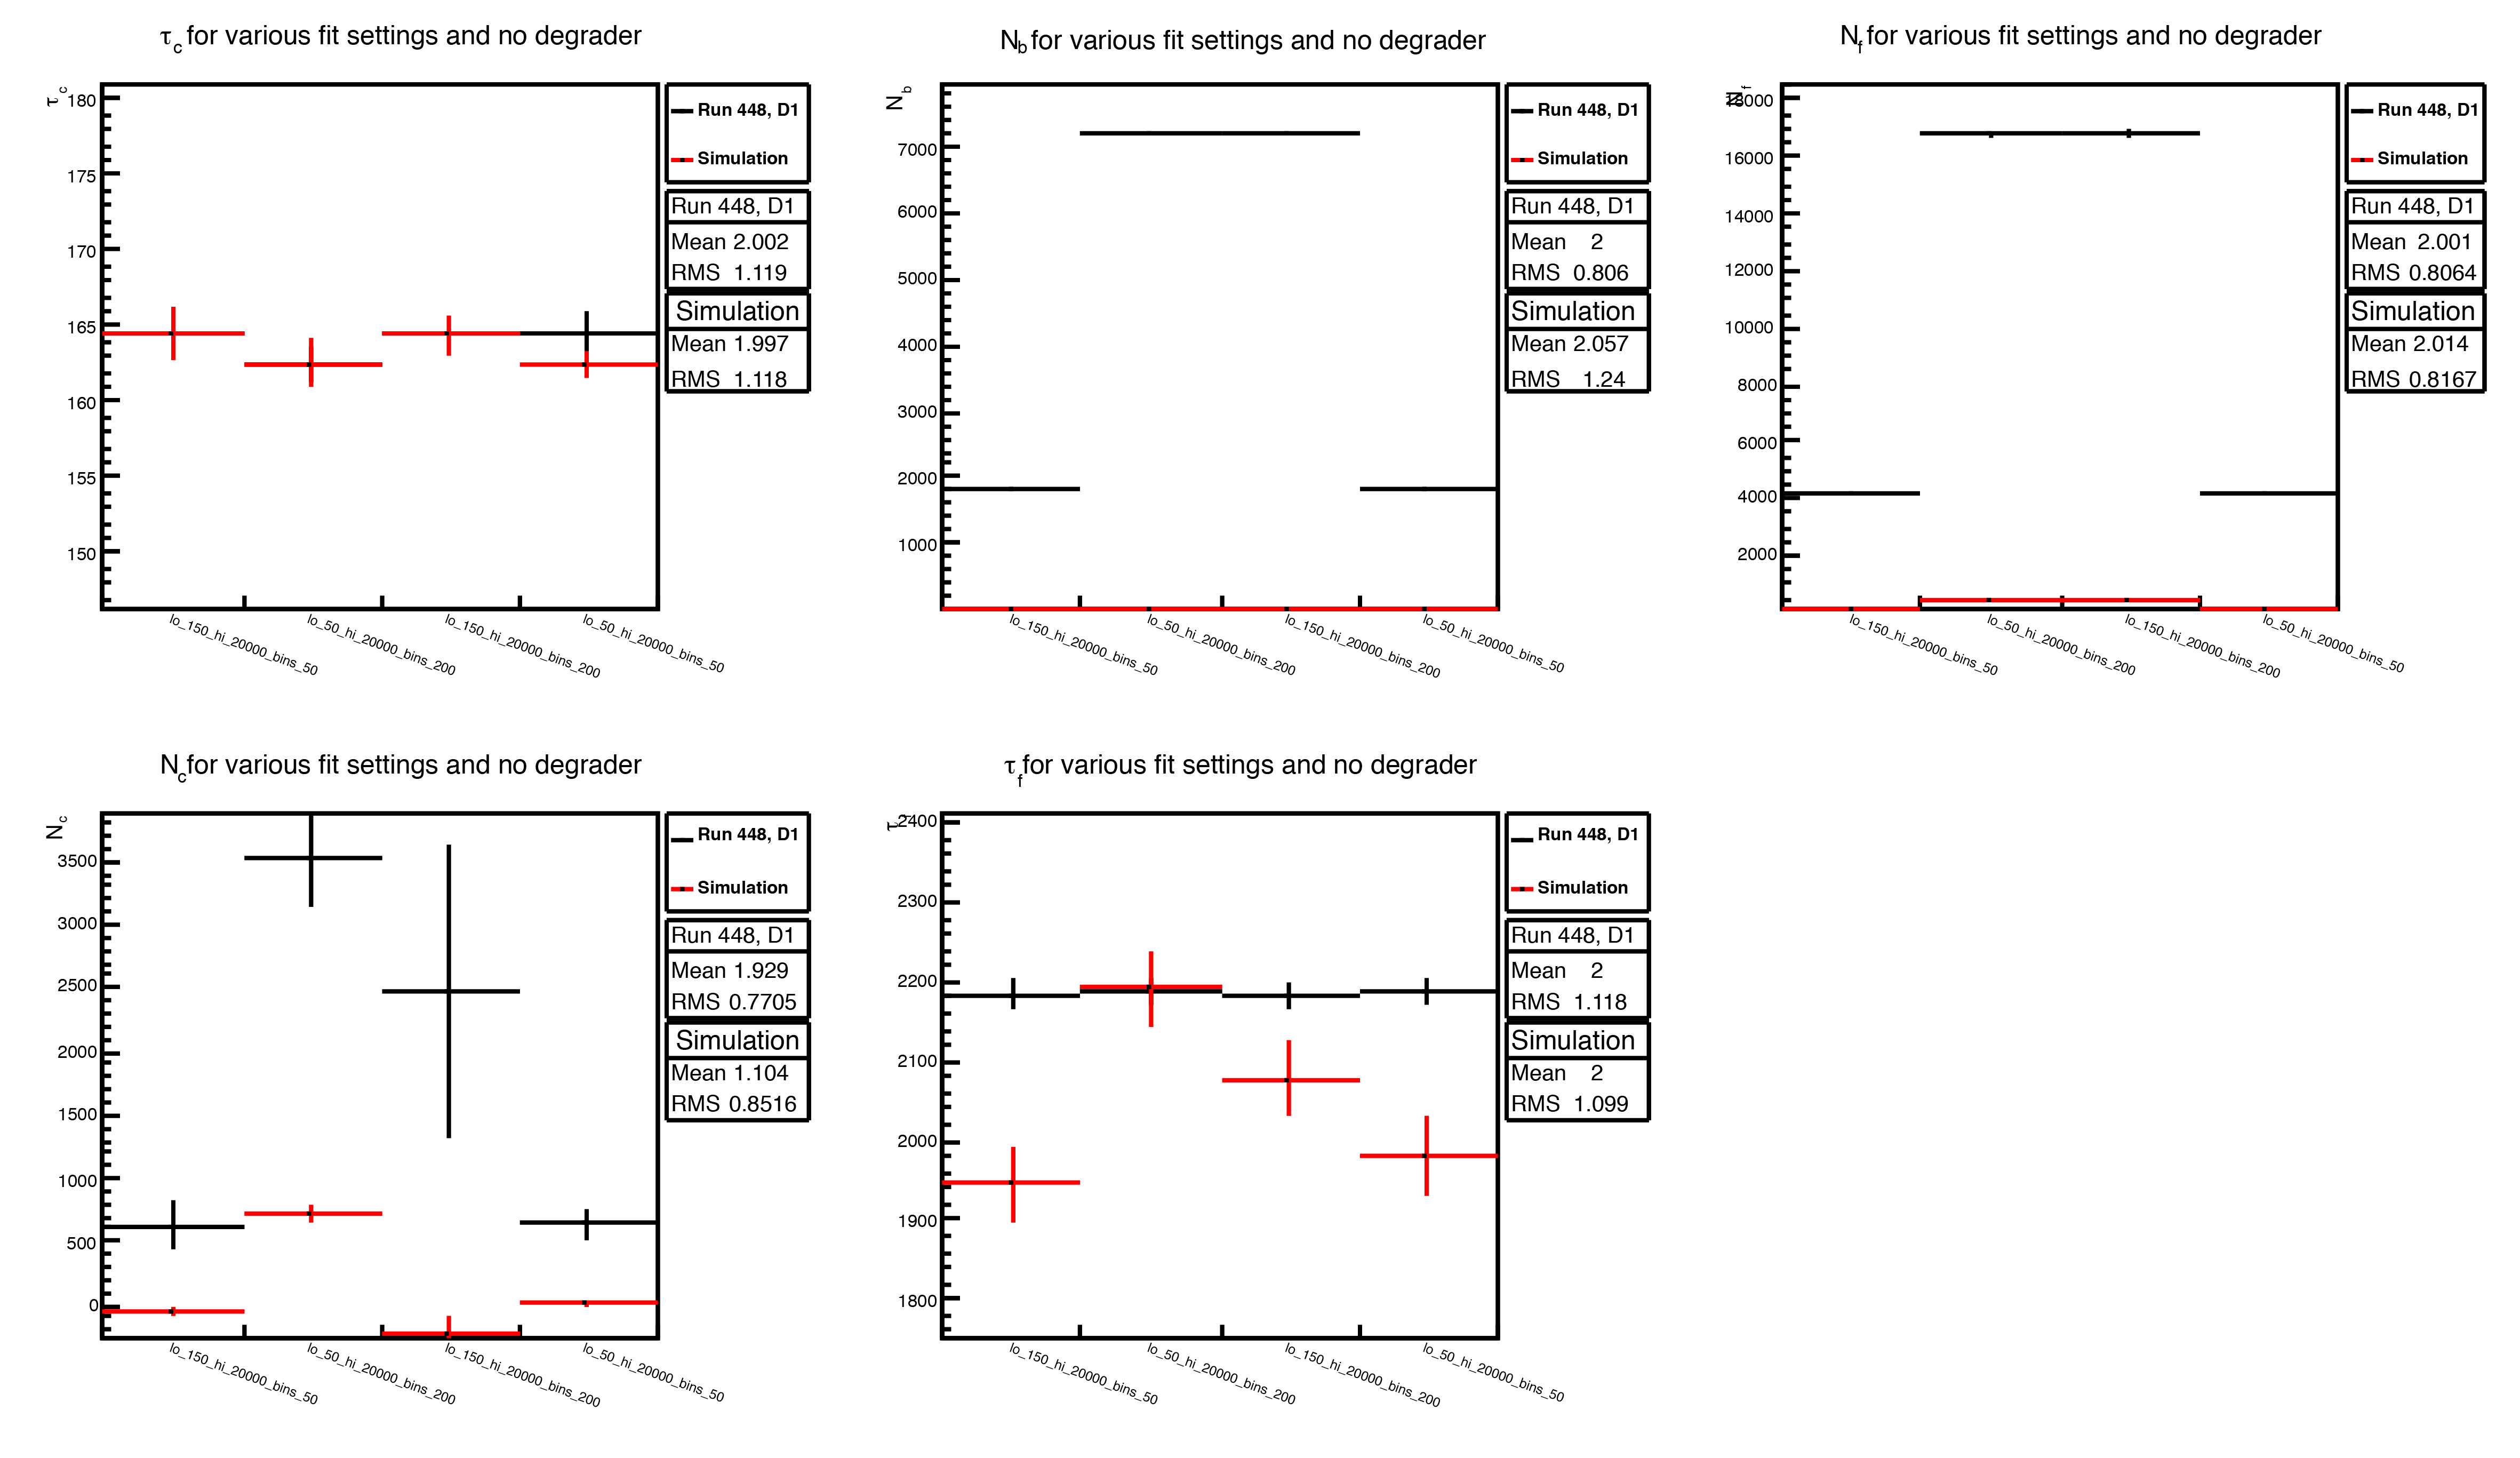
\includegraphics[width=\textwidth]{images/sim_vs_data_parameter_WRT_settings.png}
    \caption{Demonstration of the variance of fitted parameters with respect to the initial fit settings. The x axis labels list the settings used for that bin e.g. `lo\_100\_hi\_20000\_bins\_50' corresponds to a lower bound of 100~ns, an upper bound of 2\mus{} and a bin width of 50~ns. Bare in mind that the $N$ values have not had any compensation for acceptance etc. applied so difference between simulation and data is expected.}
    \label{fig:image_sim_vs_data_parameter_WRT_settings}
\end{figure}

The largest changes to the fit are due to the fit settings figure~\ref{fig:example_fits_data_and_sim} shows examples of simulated and real data with their respective fits . These determine the range that is fitted and the smoothness of the data that the fit is attempted on. The lower bound of the range probably has the largest affect on the fit. It is obvious that a large enough lower bound will utterly remove the region in which the copper component is dominant (i.e.\ $\lesssim$ 200~ns), to avoid this the minimum value of 50~ns is usually chosen which corresponds to the maximum anti-coincidence period of the trigger. The upper bound has very little affect for any reasonable value ($>$15\mus) as that portion of the histograms is usually flat. The bin width has an important part to play as it the prime method of smoothing data. 

\begin{figure}[htbp]
    \centering
        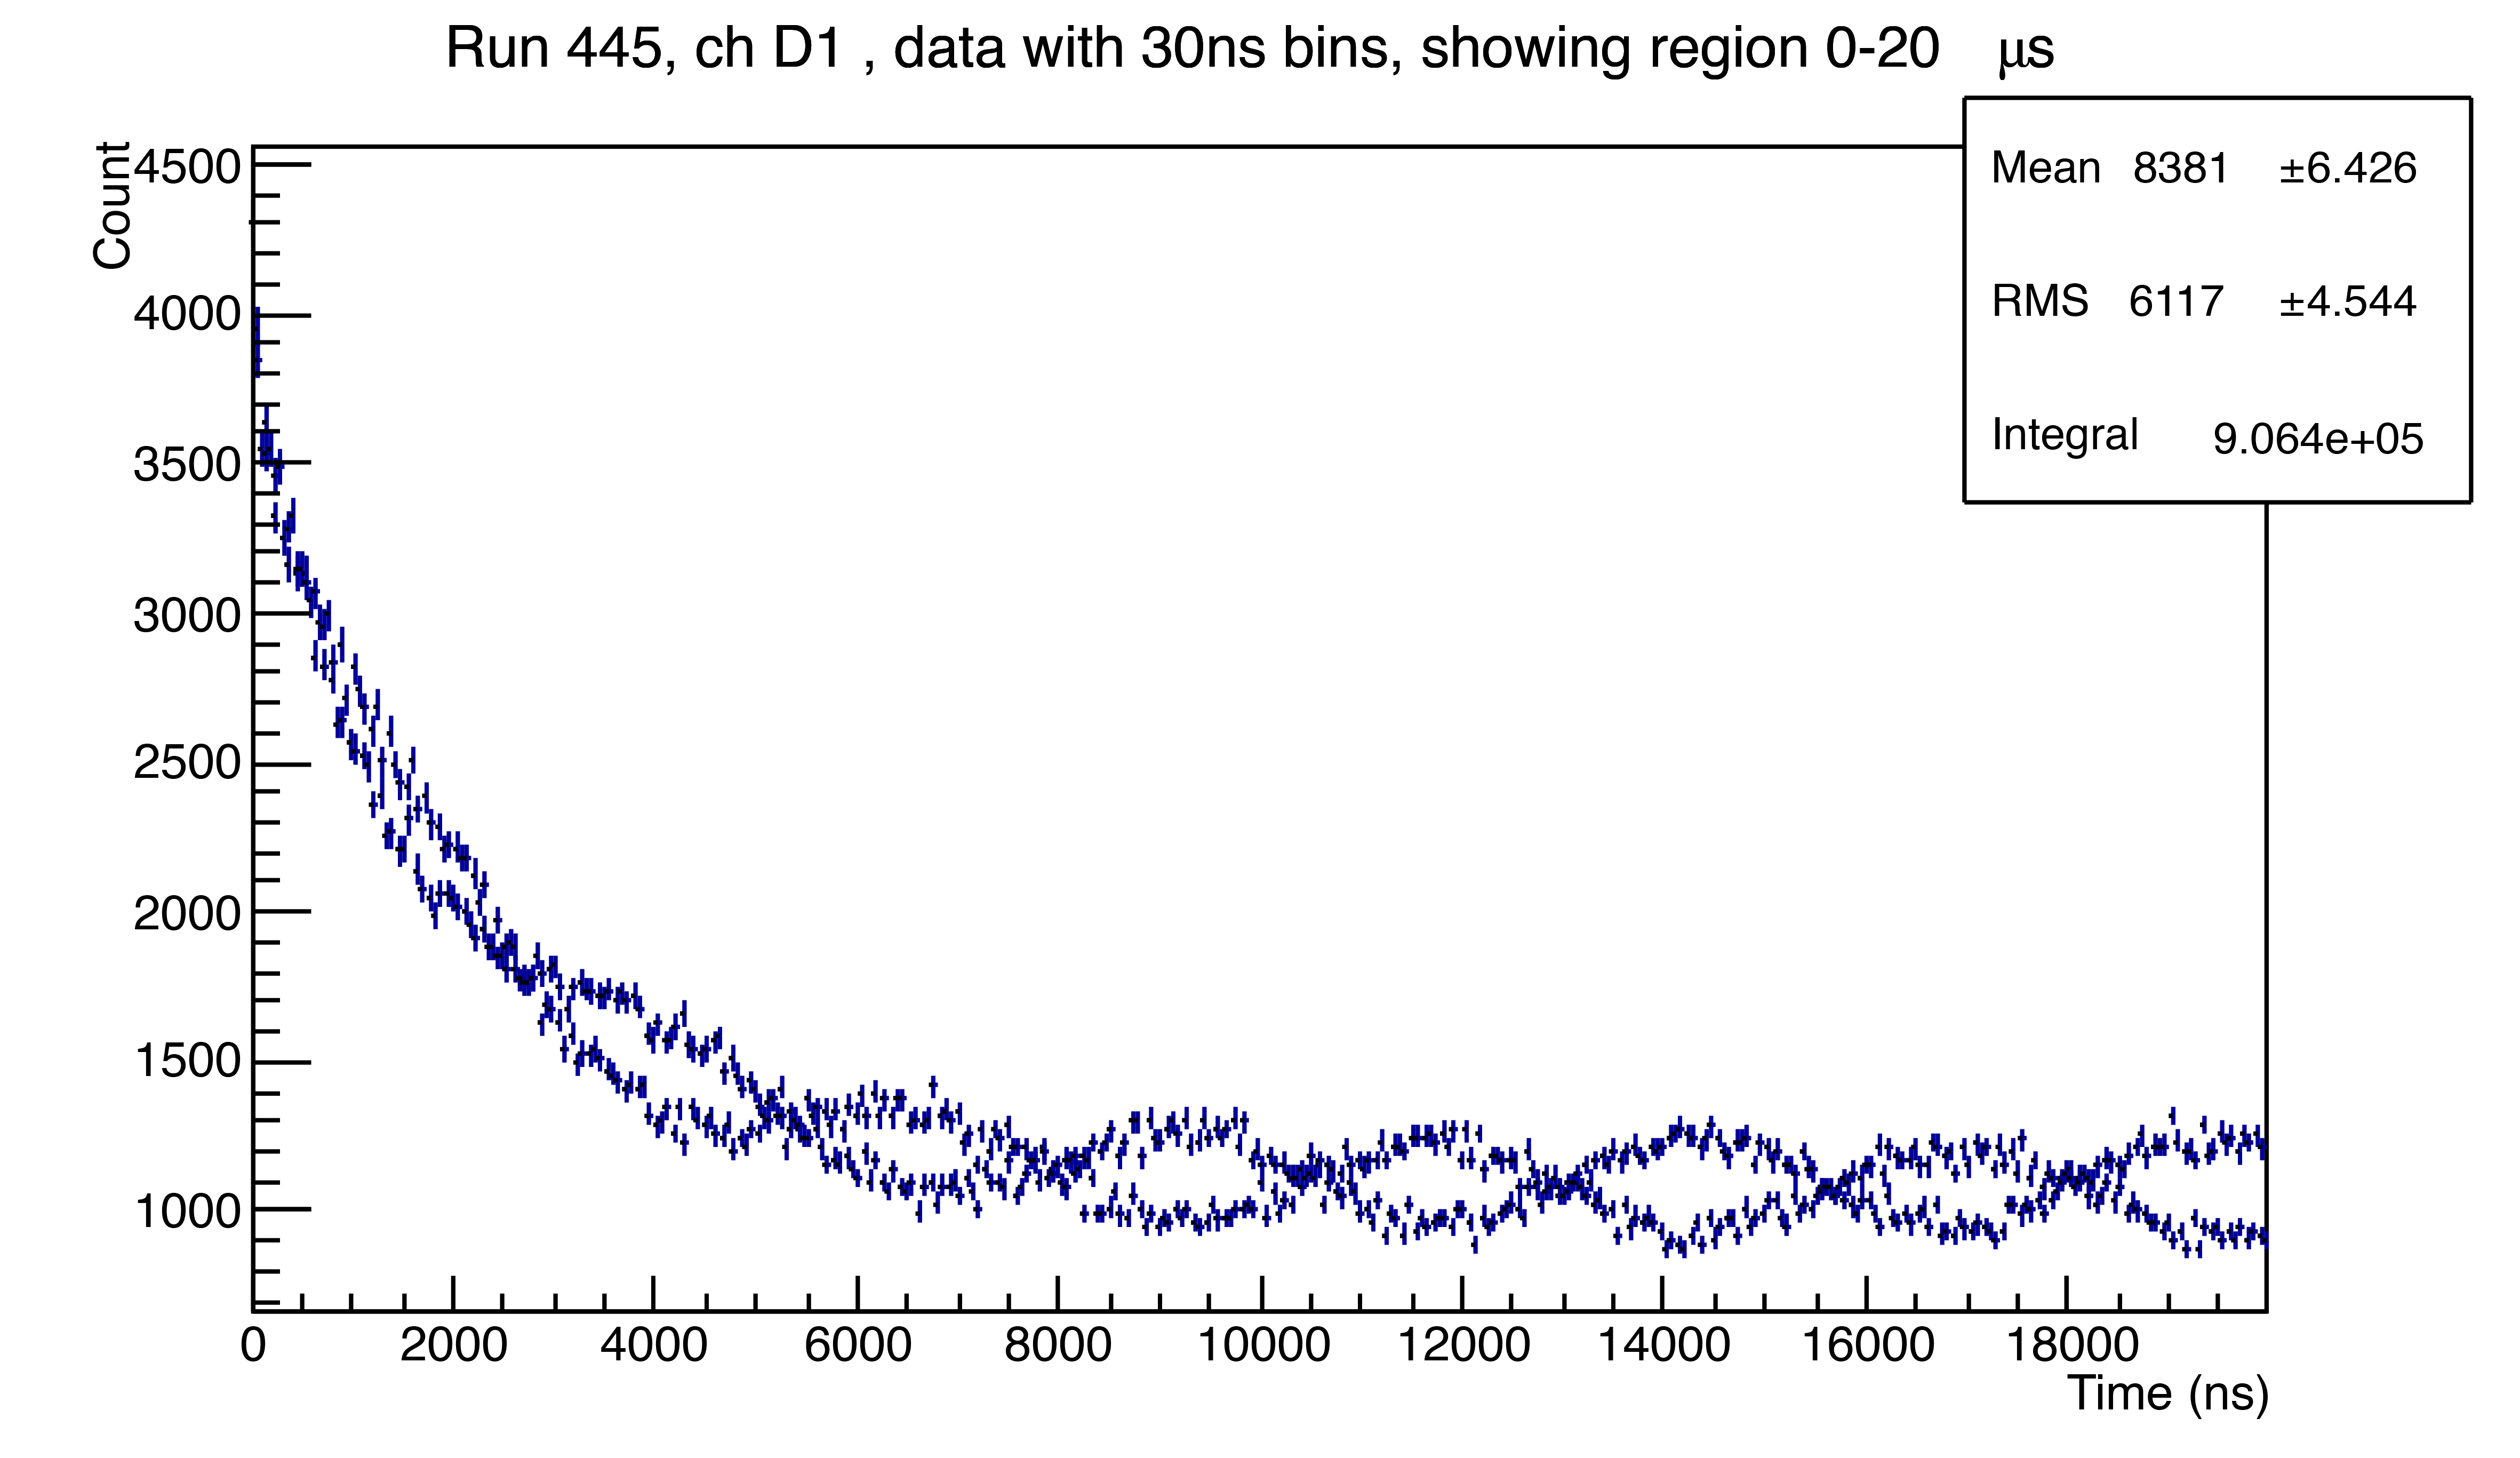
\includegraphics[width=\textwidth]{images/example_noise.png}
    \caption{Example of the noise seen in the data. Both the high ($\sim$16~MHz) and low ($\sim$45~kHz) frequency components are clearly visible. An enlarged view of the tail of this distribution is given in figure~\ref{fig:example_noise_zoom}}
    \label{fig:example_noise}
\end{figure}
%
\begin{figure}[htbp]
    \centering
        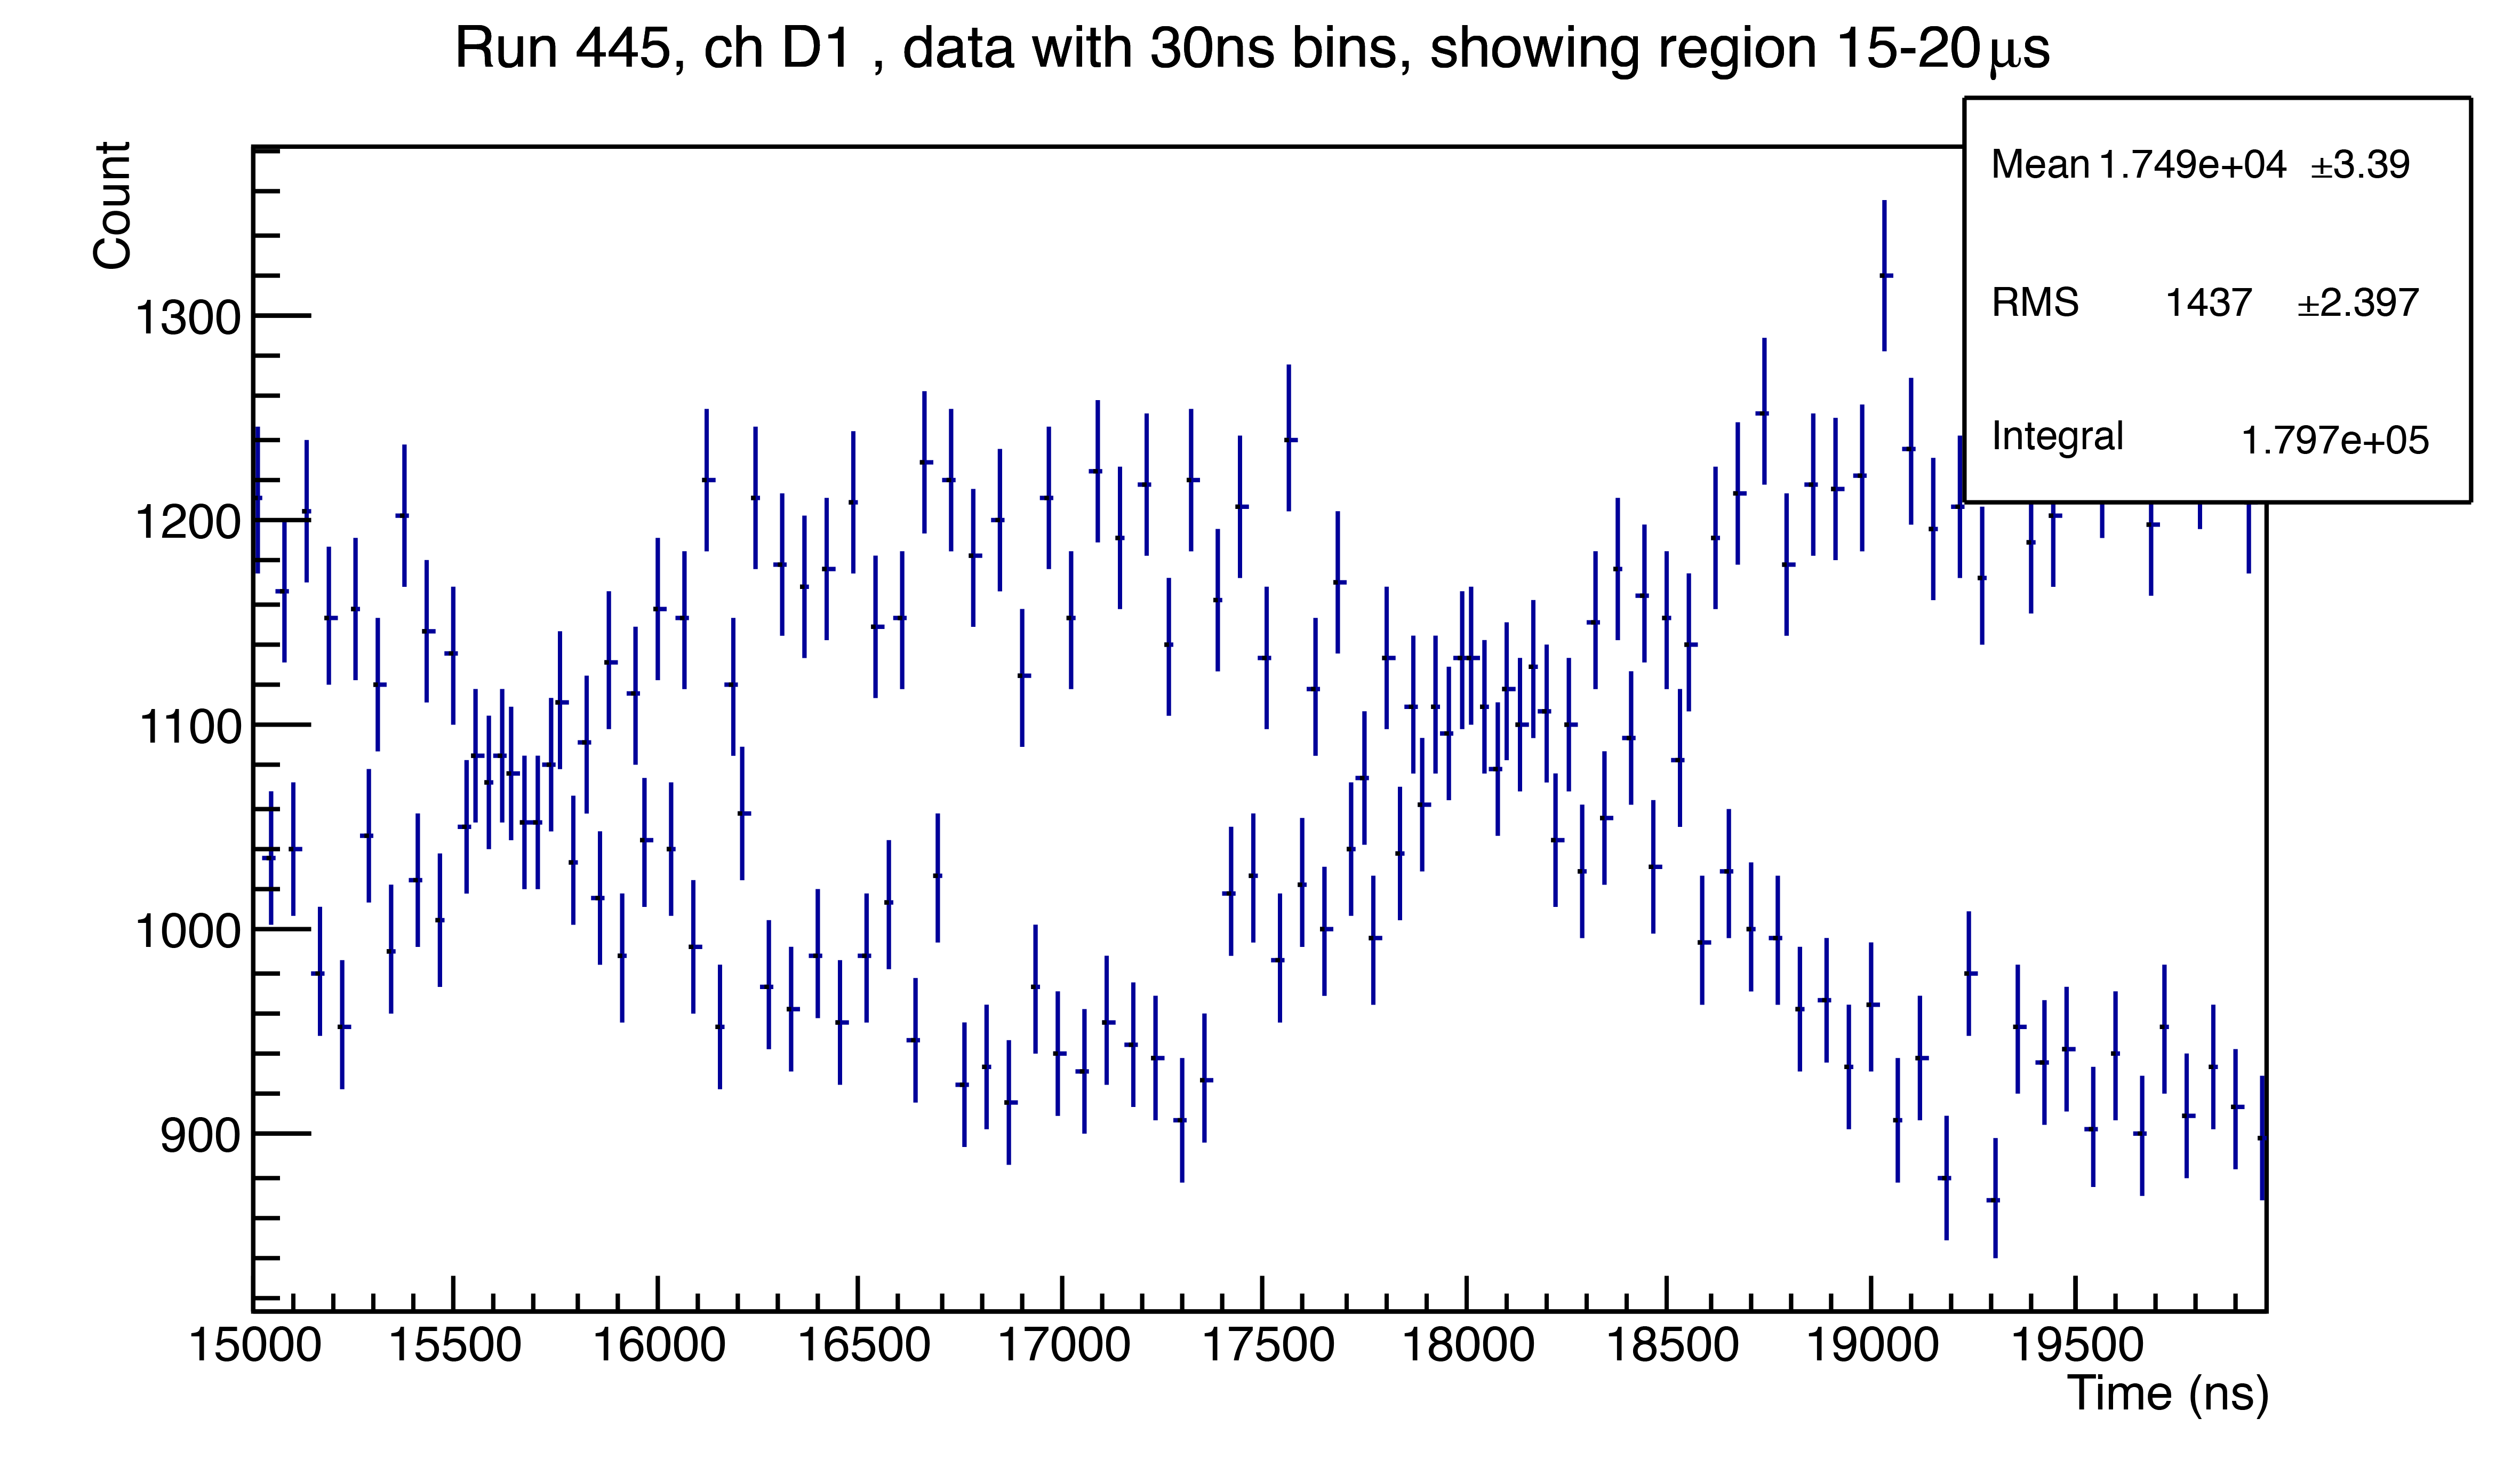
\includegraphics[width=\textwidth]{images/example_noise_zoom.png}
    \caption{Enlarged view showing the high frequency component of the noise more clearly.}
    \label{fig:example_noise_zoom}
\end{figure}

Smoothing the data appears to be very important judging by the noise seen in figure~\ref{fig:example_noise}. As can be seen there appears to be a high frequency component with a period $\sim$60~ns (frequency $\sim$16~MHz) imposed upon a much slower carrier period $\sim$2.2\mus{} (frequency $\sim$45~kHz). Using a suitable bin width (e.g. 100~ns) the high frequency component can be removed and the overall affect of the noise greatly reduced (see figure~\ref{fig:example_smoothing}).

\begin{figure}[htbp]
    \centering
        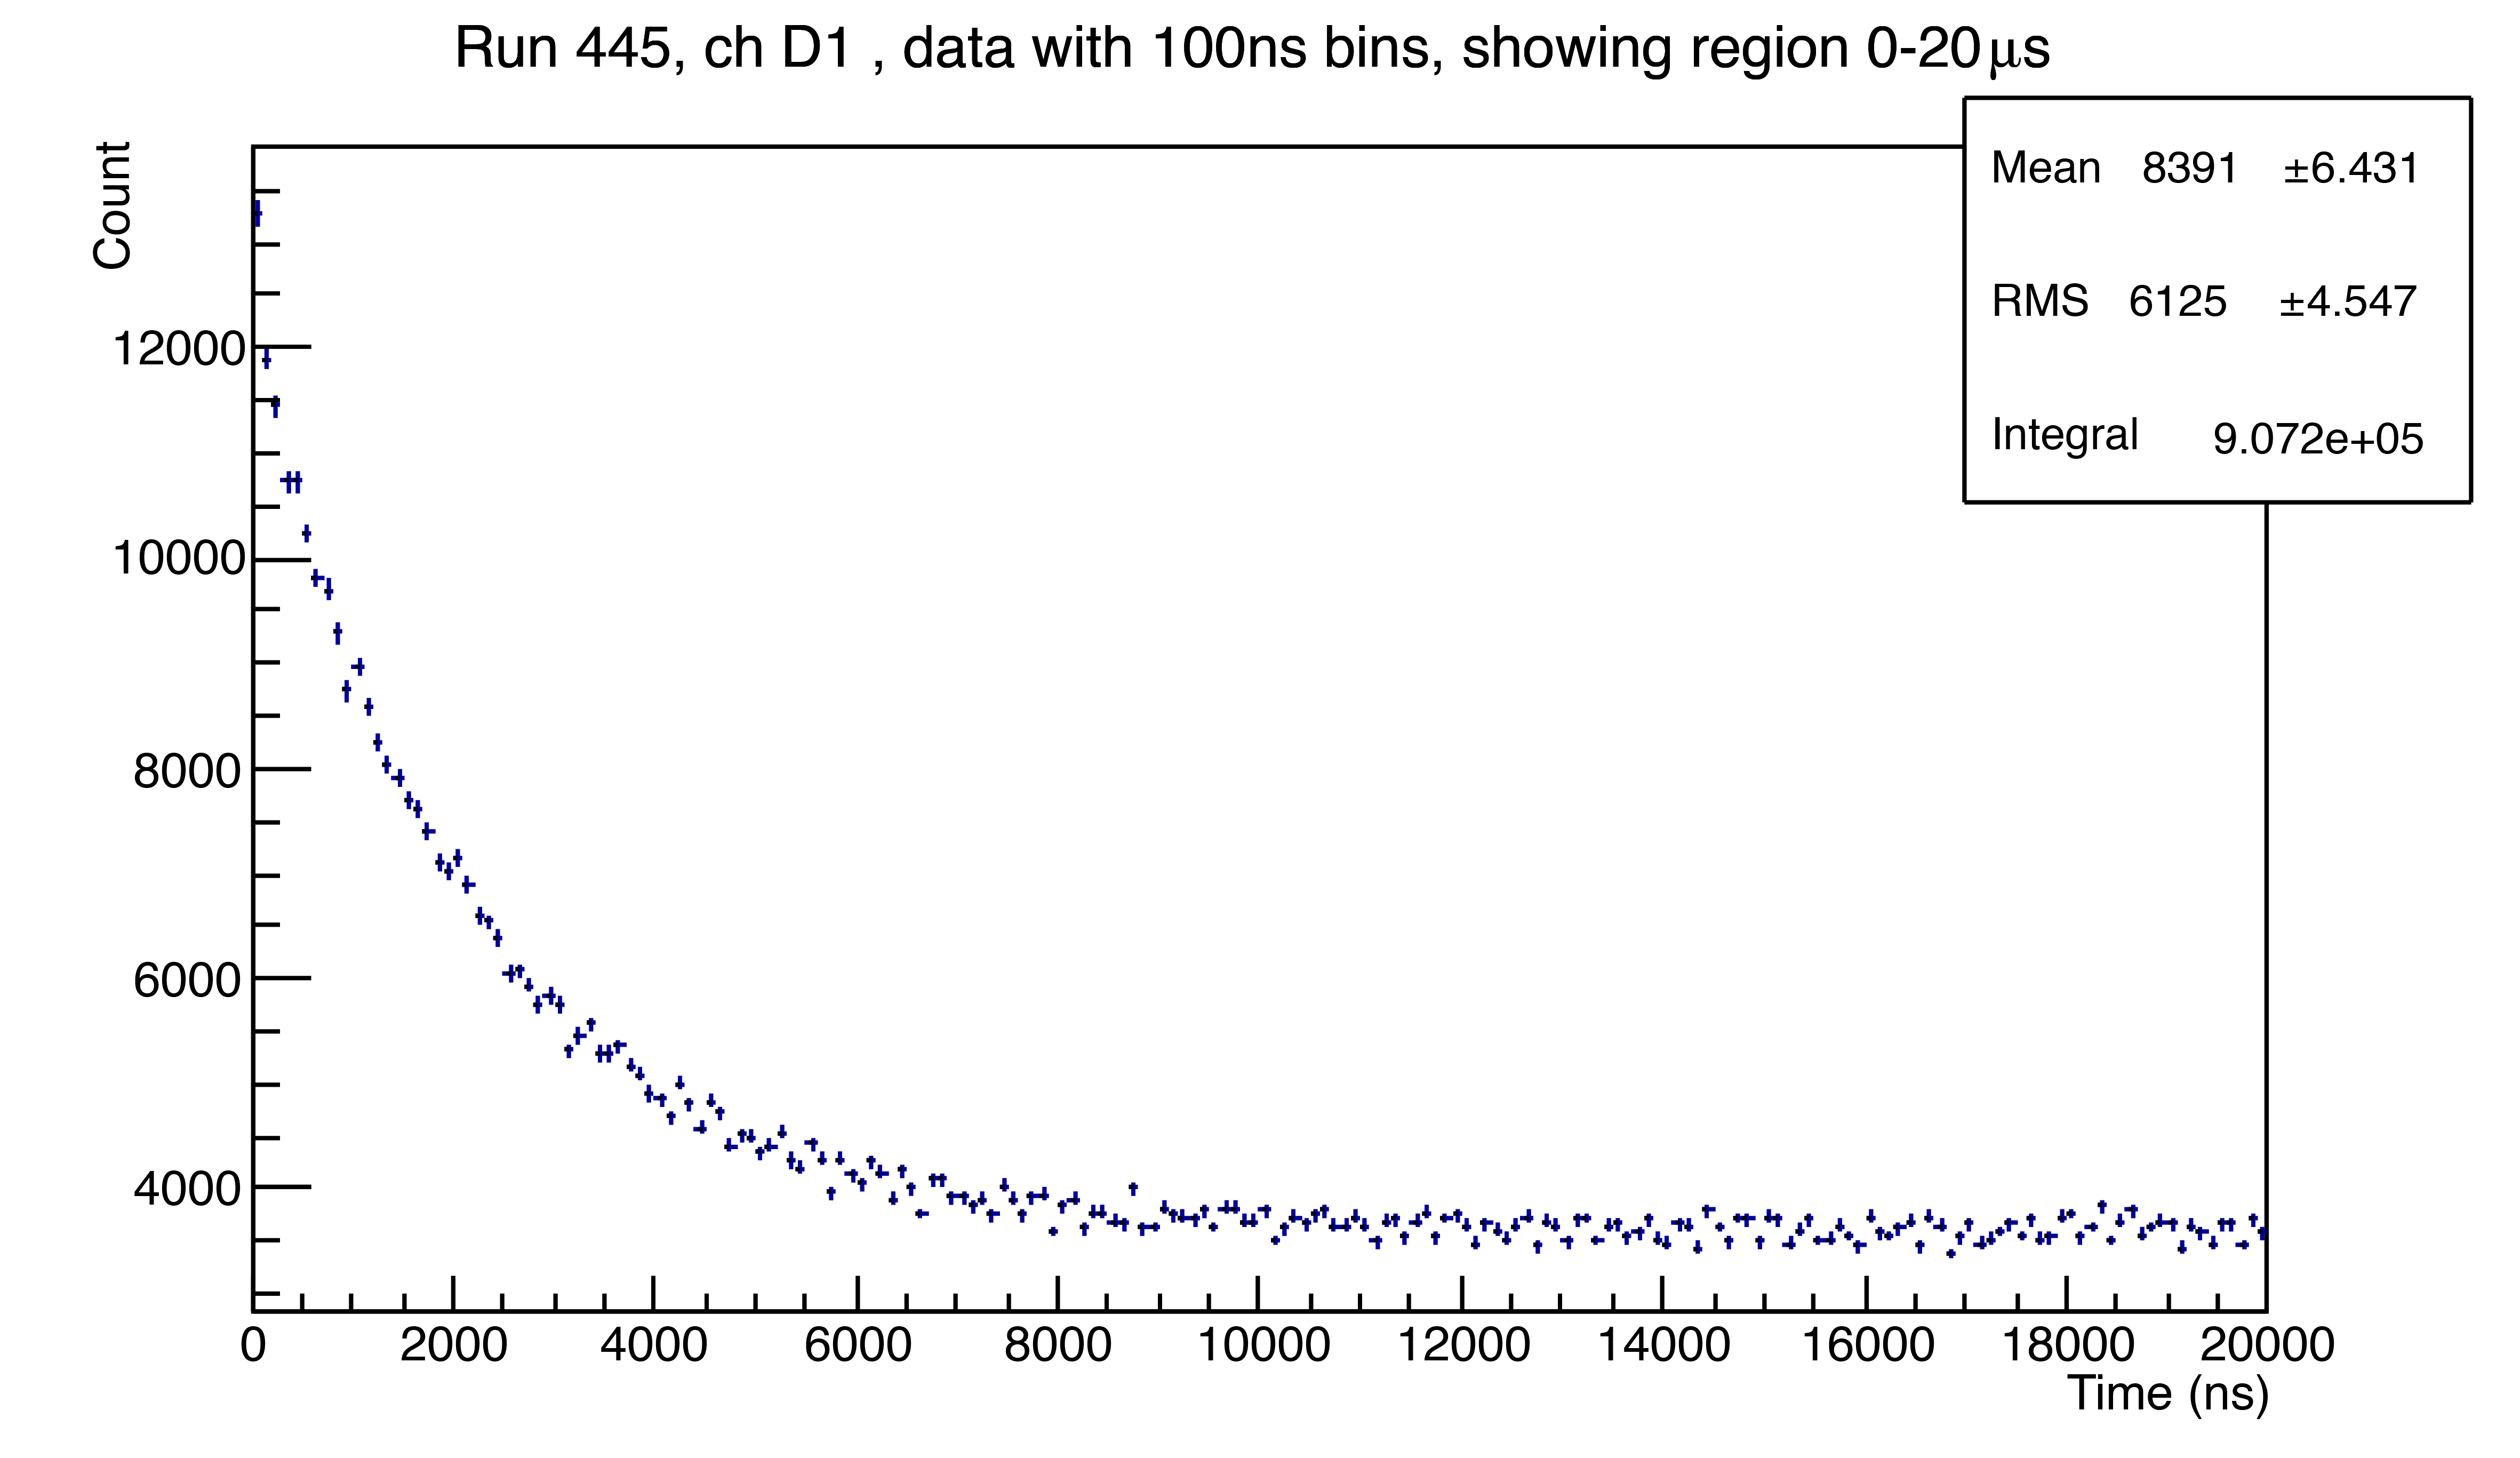
\includegraphics[width=\textwidth]{images/example_smoothing.png}
    \caption{Example of the data once suitably large bins (in this case 100~ns) have been applied in order to remove high frequency noise cf.\ figure~\ref{fig:example_noise}.}
    \label{fig:example_smoothing}
\end{figure}

The initial fit parameters were set by `eyeball' to approximations of their expected value, if this were not done ROOT would set all values to 0. A reasonably large range of values was chosen to avoid degeneracies (this is especially important to make sure that each fit corresponds to its label). $\tau_{c}$ is generally fixed to a range of $\pm$1~ns about its canonical value of 163.5~\cite{PhysRevC.35.2212} as this is a known value reasonably different compared to the other muonic lifetimes\footnote{The lifetimes for the other major materials in the detector are: Hydrogen 2194.903$\pm$0.066, Carbon 2026.3$\pm$1.5~ns, Nitrogen 1906.8$\pm$3.0~ns, Oxygen 1795.4$\pm$2~ns~\cite{PhysRevC.35.2212}. Where the scintillator is assumed to be mostly carbon and hydrogen and the air mainly nitrogen and oxygen.}. It is worth noting that only the negatively charged muons can form muonic atoms and so the copper component of the fit makes a reasonable approximation to this number whilst the free component will be composed of primarily of positively as well as negatively charged muons.

Once the histograms were fitted the fit parameters were extracted and used to create sub-functions corresponding to the individual components. Using ROOT's `Integral' and `IntegralError' functions the number of decays for each channel corresponding to each component could then be calculated. Equally summing over all the channels in a run the total number of muons for that run could be calculated.
% subsection the_implementation (end)
% section fitting_and_integration (end)
%%%%%%%%%%%%%%%%%%%%%%%%%%%%%%%%%%%%%%%%%%%%%%%%%%%%%%%%%%%%%%%%%%%%%%%%%%%%%%
\section{Muon Yield} % (fold)
\label{sec:muon_yield}
Once the number of muons for each run is known the muon yield is ultimately a matter of scaling. The formula used is:
\begin{align}
    Y = \frac{N_{mu}}{\epsilon \times A \times D \times t_{r} \times I}
\end{align}
Where $Y$ is the yield, $N_{mu}$ the number of muons for that run, $\epsilon$ is the detector efficiency, $A$ the acceptance for that degrader thickness, $D$ is the dead-time, $t_{r}$ is the run time in seconds and $I$ is the proton current. The detector efficiency was not measured for this experiment but based on previous experiments (e.g. detector efficiency for MuSIC~3) is set to 50\% and incorporated into both calculations for simulated and real data. 
% chapter muon_momentum_spectrum (end)
%%%%%%%%%%%%%%%%%%%%%%%%%%%%%%%%%%%%%%%%%%%%%%%%%%%
% part characterising_the_beam (end)
%%%%%%%%%%%%%%%%%%%%%%%%%%%%%%%%%%%%%%%%%%%%%%%%%%%
